% SPARTAN-16 CPU design report.
% Build it with:  make report
\documentclass[10pt]{article}
\usepackage[letterpaper, margin=0.75in, top=0.7in, bottom=0.8in]{geometry}
\usepackage[T1]{fontenc}
\usepackage{lmodern}
\usepackage{microtype}
\usepackage[table]{xcolor}
\usepackage{tikz}
\usetikzlibrary{arrows.meta, positioning, shapes.geometric, calc}
\usepackage{booktabs, tabularx, array, longtable}
\usepackage{caption}
\usepackage{fancyhdr}
\usepackage{titlesec}
\usepackage{listings}
\usepackage{tcolorbox}
\usepackage[hidelinks]{hyperref}

\newcommand{\sampleSteps}{19}\newcommand{\sampleCycles}{65}\newcommand{\sampleOut}{6}\newcommand{\sampleWords}{11}
\newcommand{\factSteps}{44}\newcommand{\factCycles}{150}\newcommand{\factOut}{40320}\newcommand{\factWords}{11}
\newcommand{\powerSteps}{42}\newcommand{\powerCycles}{150}\newcommand{\powerOut}{64}\newcommand{\powerWords}{40}

% Put the team names and the work each person did here.
% After editing, build the PDF again with:  make report

\newcommand{\teamnames}{%
  Vineet Kumar \\
  Sakshat Nandkumar Patil \\
  Aishwarya Madhave
}

% One row per person:   Name & what they did \\ \midrule
\newcommand{\teamcontributions}{%
  Vineet Kumar &
    Designed the instruction set: opcodes, the 8 instruction formats, the branch conditions
    and the ISA lookup table (\texttt{src/isa.c}). Wrote the CPU parts in \texttt{src/components.c}
    (registers, ALU and flags, buses, RAM, control unit) and the fetch, decode, execute loop in
    \texttt{src/cpu.c}. Wrote the 3! sample and the 8! program in assembly. \\ \midrule
  Sakshat Nandkumar Patil &
    Wrote the assembler (\texttt{src/assembler.c}), the loader that writes the program into RAM
    over the bus (\texttt{src/loader.c}), the trace printer (\texttt{src/display.c}) and the
    tests (\texttt{tests/test\_spartan.c}). \\ \midrule
  Aishwarya Madhave &
    Wrote the \texttt{s16cc} C compiler (\texttt{src/compiler.c}) and the C program \texttt{power.c}.
    Drew the CPU block diagram (Figure~\ref{fig:cpu}). Put together this report and the program
    that makes its tables (\texttt{report/gen\_report.c}). \\
}


% ---------- colors ----------
\definecolor{frame}{HTML}{1F3A5F}
\definecolor{boxc}{HTML}{E8F0FA}
\definecolor{muxc}{HTML}{FFF4D6}
\definecolor{aluc}{HTML}{FDE2D2}
\definecolor{memc}{HTML}{E3F4E1}
\definecolor{cpuc}{HTML}{F7F9FC}
\definecolor{busc}{HTML}{1F3A5F}
\definecolor{ctlc}{HTML}{C0392B}
\definecolor{opc}{HTML}{BFD7F2}
\definecolor{fld}{HTML}{F4F6F9}
\definecolor{fixed}{HTML}{E2E2E2}
\definecolor{wrt}{HTML}{C0392B}
\definecolor{pcc}{HTML}{9BE39B}
\definecolor{datac}{HTML}{DCEBFA}
\definecolor{stackc}{HTML}{FFF0C2}
\definecolor{outc}{HTML}{FFE08A}
\definecolor{dim}{HTML}{7A8794}
\definecolor{funcc}{HTML}{E8F0FA}

% figures and tables stay where we put them (no floating)
\makeatletter
\newenvironment{tablehere}{\par\vspace{8pt}\noindent\begin{minipage}{\linewidth}\centering\def\@captype{table}}{\end{minipage}\par\vspace{8pt}}
\newenvironment{figurehere}{\par\vspace{8pt}\noindent\begin{minipage}{\linewidth}\centering\def\@captype{figure}}{\end{minipage}\par\vspace{8pt}}
% table rows are read with the plain TeX \input so \bottomrule can follow them
\let\rawinput\@@input
\makeatother

% ---------- page numbers like 03/20 ----------
\makeatletter
\newcommand{\twodigit}[1]{\ifnum#1<10 0\fi\number#1}
\providecommand{\lastpage}{0}
\AtEndDocument{\clearpage\immediate\write\@auxout{\gdef\string\lastpage{\the\numexpr\value{page}-1\relax}}}
\makeatother
\pagestyle{fancy}
\fancyhf{}
\renewcommand{\headrulewidth}{0.4pt}
\fancyhead[L]{\sffamily\small SPARTAN-16 CPU Design}
\fancyhead[R]{\sffamily\small CMPE 220}
\fancyfoot[C]{\sffamily\small \twodigit{\value{page}}/\twodigit{\lastpage}}
\fancypagestyle{plain}{\fancyhf{}\renewcommand{\headrulewidth}{0pt}%
  \fancyfoot[C]{\sffamily\small \twodigit{\value{page}}/\twodigit{\lastpage}}}

% ---------- headings and captions ----------
\titleformat{\section}{\sffamily\Large\bfseries\color{frame}}{\thesection}{0.6em}{}[{\color{frame}\titlerule}]
\titleformat{\subsection}{\sffamily\large\bfseries\color{frame}}{\thesubsection}{0.5em}{}
\titlespacing*{\section}{0pt}{10pt}{6pt}
\titlespacing*{\subsection}{0pt}{8pt}{4pt}
\captionsetup{font={small,sf}, labelfont=bf, skip=4pt}
\setlength{\parindent}{0pt}
\setlength{\parskip}{3pt}

\lstdefinestyle{csrc}{language=C, basicstyle=\ttfamily\small, keywordstyle=\color{frame}\bfseries,
  commentstyle=\color{dim}\itshape, numbers=left, numberstyle=\tiny\color{dim}, frame=single,
  rulecolor=\color{frame!40}, backgroundcolor=\color{fld}, xleftmargin=1.5em, framexleftmargin=1.5em,
  columns=fullflexible, keepspaces=true}

% ---------- one step of a trace ----------
\tcbset{stepbox/.style={width=0.497\textwidth, nobeforeafter, box align=top,
  colback=white, colframe=frame, coltitle=white, fonttitle=\ttfamily\footnotesize\bfseries,
  fontupper=\ttfamily\footnotesize, boxrule=0.5pt, arc=1.2pt, left=3pt, right=3pt, top=2pt,
  bottom=2pt, toptitle=1pt, bottomtitle=1pt}}

\newcommand{\legend}{%
  \begin{tcolorbox}[colback=fld, colframe=frame!40, boxrule=0.4pt, arc=1pt, left=4pt, right=4pt,
    top=2pt, bottom=2pt, fontupper=\small\sffamily]
  \textbf{One box = the CPU and RAM after one instruction.}
  \textbf{F}, \textbf{D}, \textbf{E} = fetch, decode, execute, one clock tick each.
  \textcolor{wrt}{\textbf{Red register}} = just changed. [ASCII] = the value as characters, one per byte (. = not printable).\\[2pt]
  RAM rows:\;
  \colorbox{pcc}{\strut next instruction (PC)}\quad
  \colorbox{wrt}{\strut\textcolor{white}{\textbf{just written}}}\quad
  \colorbox{datac}{\strut data}\quad
  \fcolorbox{dim}{white}{\strut code}
  \end{tcolorbox}}

\begin{document}

% =====================================================================
\begin{titlepage}
\thispagestyle{plain}
\centering
\vspace*{1.2in}
{\sffamily\bfseries\color{frame}\fontsize{38}{44}\selectfont SPARTAN-16\par}
\vspace{8pt}
{\sffamily\Large Our own 16-bit CPU, simulated in C\par}
\vspace{18pt}
{\color{frame}\rule{0.6\textwidth}{1pt}\par}
\vspace{18pt}
{\large CMPE 220 CPU Design Project\par}
\vspace{14pt}
{\normalsize Code: \url{https://github.com/vineetkia/CMPE-220-CPU-Simulation-Project}\par}
\vspace{0.9in}
{\sffamily\large\bfseries Team Members\par}
\vspace{8pt}
{\large \teamnames\par}
\vfill
{\large \today\par}
\vspace{0.4in}
\end{titlepage}
\setcounter{page}{2}

% =====================================================================
\section*{Contents}
\begin{tabularx}{\textwidth}{@{}lX r@{}}
\toprule
1 & CPU design: CPU, bus and RAM & \pageref{sec:cpu}\\
2 & The CPU in our C program & \pageref{sec:struct}\\
3 & Instruction set (ISA) & \pageref{sec:isa}\\
4 & How to run & \pageref{sec:run}\\
5 & Program 1: add two numbers & \pageref{sec:add}\\
6 & Program 2: multiply two numbers using only ADD & \pageref{sec:mul}\\
7 & Results & \pageref{sec:results}\\
8 & Who did what & \pageref{sec:team}\\
\bottomrule
\end{tabularx}

\begin{tablehere}
\caption{SPARTAN-16 in short}
\label{tab:spec}
\begin{tabular}{@{}ll@{}}
\toprule
Word size & 16 bits \\
RAM & 256 words of 16 bits, addresses 0x00 to 0xFF \\
Special purpose registers & PC (8 bits), IR (16), MAR (8), MDR (16), FLAGS Z N C V \\
General purpose registers & R0 to R7, 16 bits each (R0 = 0, R7 = SP) \\
System bus & address bus (8 bits), data bus (16 bits), control bus \\
Instructions & 16 opcodes, one 16-bit word each \\
Clock & 3 ticks per instruction: fetch, decode, execute \\
Program start & put into RAM by hand at 0x00, PC starts at 0x00 \\
\bottomrule
\end{tabular}
\end{tablehere}

\begin{tablehere}
\caption{Registers}
\label{tab:regs}
\small
\begin{tabular}{@{}llll@{}}
\toprule
Kind & Register & Bits & Holds \\
\midrule
Special purpose & PC & 8 & address of the next instruction \\
 & IR & 16 & the instruction being run \\
 & MAR & 8 & the address sent to RAM \\
 & MDR & 16 & the word read from or written to RAM \\
 & FLAGS & 4 & Z zero, N negative, C carry, V overflow \\
\midrule
General purpose & R0 & 16 & always 0 \\
 & R1 to R6 & 16 & values the program works with \\
 & R7 (SP) & 16 & stack pointer \\
\bottomrule
\end{tabular}
\end{tablehere}

% =====================================================================
\clearpage
\section{CPU Design}\label{sec:cpu}

\begin{figurehere}
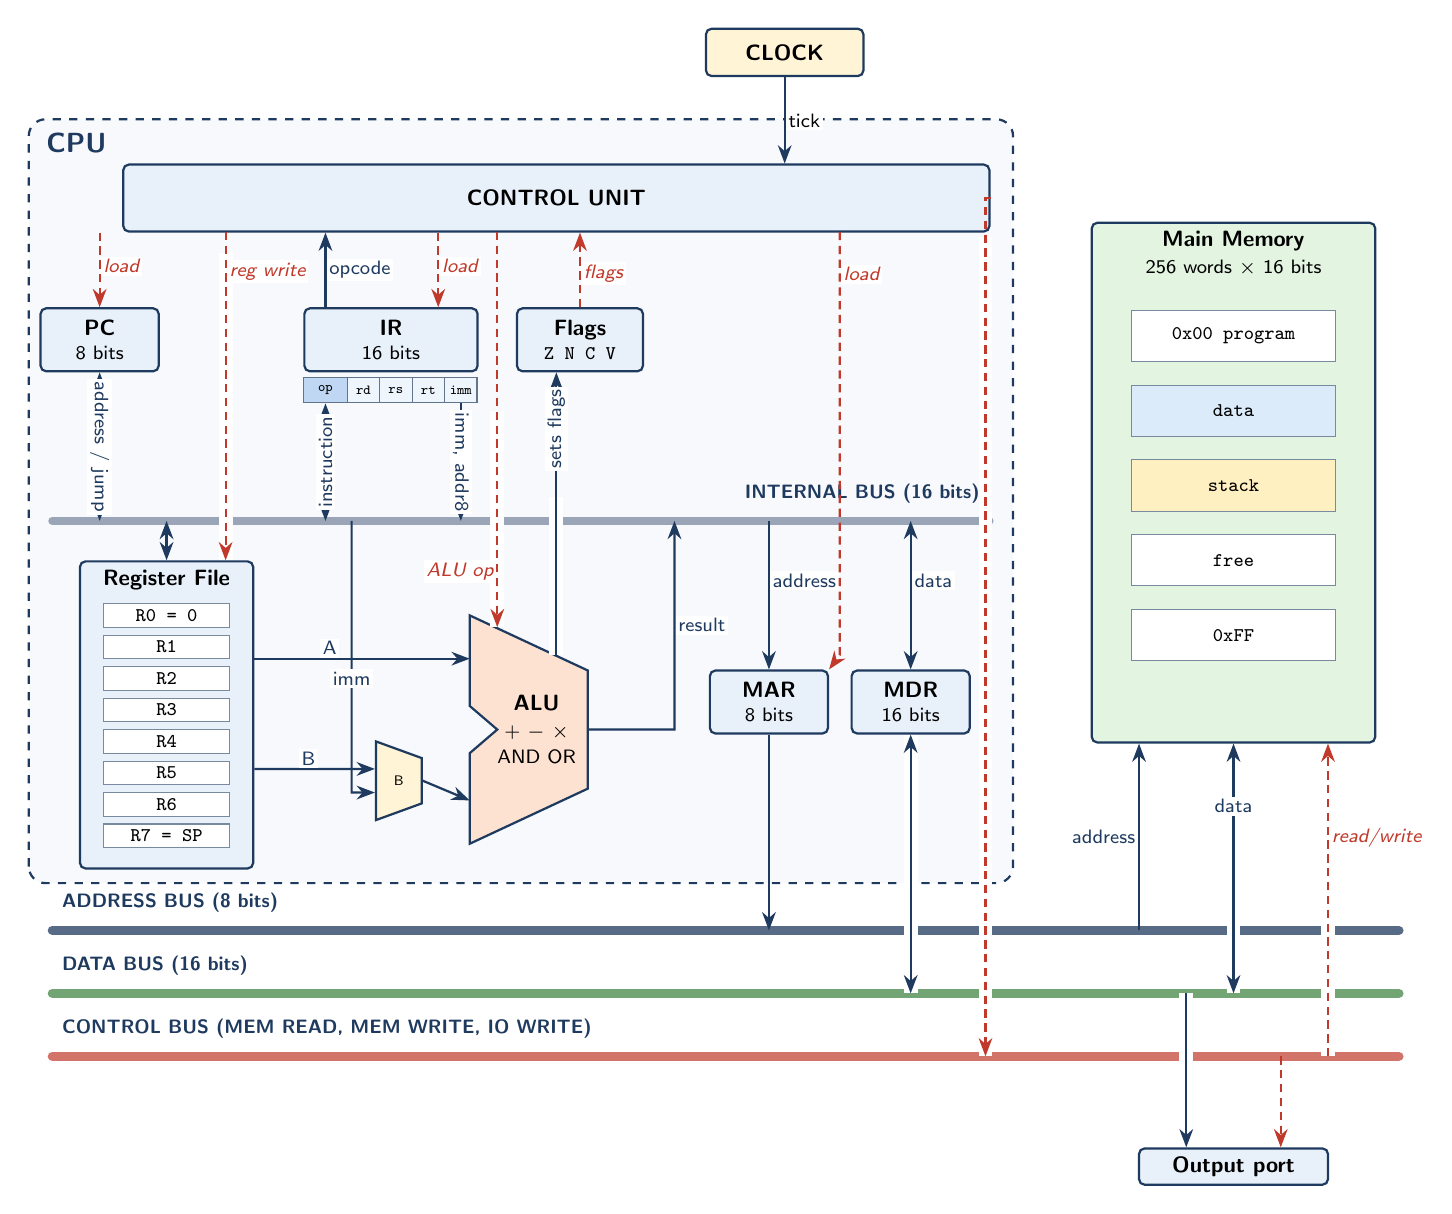
\begin{tikzpicture}[>=Stealth, font=\sffamily\footnotesize,
  blk/.style={draw=frame, thick, fill=#1, rounded corners=2pt, align=center, inner sep=3pt},
  blk/.default=boxc,
  path/.style={->, thick, draw=busc},
  bi/.style={<->, thick, draw=busc},
  ctl/.style={->, densely dashed, draw=ctlc, thick},
  halo/.style={draw=white, line width=5pt},
  lbl/.style={font=\sffamily\scriptsize, fill=white, inner sep=1pt, text=frame},
  clbl/.style={font=\sffamily\scriptsize\itshape, text=ctlc, inner sep=1pt, fill=white},
  ibus/.style={line width=3pt, draw=frame!45, line cap=round},
  sbus/.style={line width=3.4pt, draw=#1, line cap=round},
]
% ---------- CPU outline ----------
\draw[draw=frame, thick, dashed, rounded corners=6pt, fill=cpuc] (0,3.0) rectangle (12.5,12.7);
\node[anchor=north west, font=\sffamily\bfseries, text=frame] at (0.1,12.65) {CPU};

% ---------- control unit ----------
\node[blk, minimum width=11.0cm, minimum height=0.85cm] (cu) at (6.7,11.7)
  {\textbf{CONTROL UNIT}};
\node[draw=frame, thick, fill=muxc, rounded corners=2pt, minimum width=2.0cm, minimum height=0.6cm, font=\sffamily\footnotesize] (clk) at (9.6,13.55) {\textbf{CLOCK}};
\draw[->, thick, draw=frame] (clk.south) -- node[font=\sffamily\scriptsize, fill=white, inner sep=1pt, right]{tick} (clk.south |- cu.north);

% ---------- top row: PC, IR, flags ----------
\node[blk, minimum width=1.5cm, minimum height=0.8cm] (pc) at (0.9,9.9) {\textbf{PC}\\[-1pt]\scriptsize 8 bits};
\node[blk, minimum width=2.2cm, minimum height=0.8cm] (ir) at (4.6,9.9) {\textbf{IR}\\[-1pt]\scriptsize 16 bits};
\foreach \n/\w/\x/\f in {op/4/0/100, rd/3/4/25, rs/3/7/25, rt/3/10/25, imm/3/13/25} {
  \node[draw=frame!70, fill=opc!\f, minimum width=\w*0.1375cm, minimum height=0.32cm,
        inner sep=0pt, font=\ttfamily\tiny, anchor=north west] (f\n) at ($(ir.south west)+(\x*0.1375,-0.06)$) {\n};
}
\node[blk, minimum width=1.6cm, minimum height=0.8cm] (flags) at (7.0,9.9) {\textbf{Flags}\\[-1pt]\ttfamily\scriptsize Z N C V};

% ---------- internal bus ----------
\draw[ibus] (0.3,7.6) -- (12.2,7.6);
\node[font=\sffamily\scriptsize\bfseries, text=frame, anchor=south east] at (12.2,7.7) {INTERNAL BUS (16 bits)};

% ---------- bottom row: registers, ALU, MAR, MDR ----------
\node[blk, minimum width=2.2cm, minimum height=3.9cm, anchor=north] (rf) at (1.75,7.1) {};
\node[anchor=north, align=center] at (rf.north) {\textbf{Register File}};
\foreach \r [count=\i] in {R0 = 0, R1, R2, R3, R4, R5, R6, R7 = SP} {
  \node[draw=frame!60, fill=white, minimum width=1.6cm, minimum height=0.3cm, inner sep=0pt, font=\ttfamily\scriptsize]
    at ($(rf.north)+(0,-0.3-0.4*\i)$) {\r};
}
\node[draw=frame, thick, fill=muxc, trapezium, trapezium angle=70, shape border rotate=270,
      minimum width=1.0cm, minimum height=0.45cm, font=\sffamily\tiny, align=center] (bmux) at (4.7,4.3) {B};
\begin{scope}[shift={(5.6,3.5)}]
  \draw[thick, draw=frame, fill=aluc] (0,0) -- (1.5,0.7) -- (1.5,2.2) -- (0,2.9) -- (0,1.75) -- (0.35,1.45) -- (0,1.15) -- cycle;
  \node[align=center] at (0.85,1.45) {\textbf{ALU}\\\scriptsize + $-$ $\times$\\\scriptsize AND OR};
  \coordinate (aluA) at (0,2.35);
  \coordinate (aluB) at (0,0.55);
  \coordinate (aluOut) at (1.5,1.45);
  \coordinate (aluTop) at (1.1,2.4);
  \coordinate (aluCtl) at (0.4,2.7);
\end{scope}
\node[blk, minimum width=1.5cm, minimum height=0.8cm] (mar) at (9.4,5.3) {\textbf{MAR}\\[-1pt]\scriptsize 8 bits};
\node[blk, minimum width=1.5cm, minimum height=0.8cm] (mdr) at (11.2,5.3) {\textbf{MDR}\\[-1pt]\scriptsize 16 bits};

% ---------- memory and output port ----------
\node[blk=memc, minimum width=3.6cm, minimum height=6.6cm, anchor=north] (mem) at (15.3,11.4) {};
\node[anchor=north, align=center] at (mem.north) {\textbf{Main Memory}\\\scriptsize 256 words $\times$ 16 bits};
\foreach \t/\c [count=\i] in {{0x00 program}/white, {data}/datac, {stack}/stackc, {free}/white, {0xFF}/white} {
  \node[draw=frame!60, fill=\c, minimum width=2.6cm, minimum height=0.65cm, font=\ttfamily\scriptsize]
    at ($(mem.north)+(0,-0.5-0.95*\i)$) {\t};
}
\node[blk, minimum width=2.4cm] (out) at (15.3,-0.6) {\textbf{Output port}};

% ---------- system bus ----------
\draw[sbus=frame!75] (0.3,2.4) -- (17.4,2.4);
\draw[sbus=green!35!black!55] (0.3,1.6) -- (17.4,1.6);
\draw[sbus=ctlc!70] (0.3,0.8) -- (17.4,0.8);
\node[font=\sffamily\scriptsize\bfseries, text=frame, anchor=south west] at (0.3,2.5) {ADDRESS BUS (8 bits)};
\node[font=\sffamily\scriptsize\bfseries, text=frame, anchor=south west] at (0.3,1.7) {DATA BUS (16 bits)};
\node[font=\sffamily\scriptsize\bfseries, text=frame, anchor=south west] at (0.3,0.9) {CONTROL BUS (MEM READ, MEM WRITE, IO WRITE)};

% ---------- paths inside the CPU ----------
\draw[bi] (pc.south) -- node[lbl, sloped, pos=0.5]{address / jump} (pc.south |- 0,7.6);
\draw[bi] (fop.south |- 0,7.6) -- node[lbl, sloped, pos=0.5]{instruction} (fop.south);
\draw[path] (fimm.south) -- node[lbl, sloped, pos=0.5]{imm, addr8} (fimm.south |- 0,7.6);
\draw[path] (fop.north |- ir.north) -- node[lbl, right, pos=0.5]{opcode} (fop.north |- cu.south);
\draw[bi] (rf.north) -- (rf.north |- 0,7.6);
\draw[path] (rf.east |- aluA) -- node[lbl, above, pos=0.35]{A} (aluA);
\draw[path] (rf.east |- 0,4.45) -- node[lbl, above, pos=0.45]{B} ([yshift=0.15cm]bmux.west);
\draw[path] (4.1,7.6) -- (4.1,4.15) -- ([yshift=-0.15cm]bmux.west);
\node[lbl] at (4.1,5.6) {imm};
\draw[path] (bmux.east) -- (aluB);
\draw[path] (aluOut) -- (8.2,4.95) -- node[lbl, right, pos=0.5]{result} (8.2,7.6);
\draw[halo] (aluTop) -- (aluTop |- 0,7.9);
\draw[path] (aluTop) -- node[lbl, sloped, pos=0.8]{sets flags} (aluTop |- flags.south);
\draw[path] (9.4,7.6) -- node[lbl, right, pos=0.4]{address} (mar.north);
\draw[bi] (11.2,7.6) -- node[lbl, right, pos=0.4]{data} (mdr.north);

% ---------- CPU to system bus ----------
\draw[path] (mar.south) -- (mar.south |- 0,2.4);
\draw[halo] (mdr.south) -- (mdr.south |- 0,1.6);
\draw[bi] (mdr.south) -- (mdr.south |- 0,1.6);
\draw[halo] (12.15,11.2) -- (12.15,0.8);
\draw[ctl] (cu.east) -| (12.15,0.8);

% ---------- memory and output port on the system bus ----------
\draw[path] (14.1,2.4) -- node[lbl, left, pos=0.5]{address} (mem.south -| 14.1,0);
\draw[halo] (15.3,1.6) -- (15.3,2.6);
\draw[bi] (15.3,1.6) -- node[lbl, pos=0.75]{data} (mem.south -| 15.3,0);
\draw[halo] (16.5,0.8) -- (16.5,2.6);
\draw[ctl] (16.5,0.8) -- node[clbl, right, pos=0.7]{read/write} (mem.south -| 16.5,0);
\draw[halo] (14.7,1.6) -- (14.7,0.6);
\draw[path] (14.7,1.6) -- (out.north -| 14.7,0);
\draw[ctl] (15.9,0.8) -- (out.north -| 15.9,0);

% ---------- control signals inside the CPU ----------
\draw[ctl] (pc.north |- cu.south) -- node[clbl, right, pos=0.45]{load} (pc.north);
\draw[ctl] ([xshift=0.6cm]ir.north |- cu.south) -- node[clbl, right, pos=0.45]{load} ([xshift=0.6cm]ir.north);
\draw[ctl] (flags.north) -- node[clbl, right, pos=0.45]{flags} (flags.north |- cu.south);
\draw[halo] (2.5,11.0) -- (2.5,7.1);
\draw[ctl] (2.5,11.27) -- node[clbl, right, pos=0.12]{reg write} (2.5,7.1);
\draw[halo] (5.95,9.0) -- (5.95,6.25);
\draw[ctl] (5.95,11.27) -- node[clbl, left, pos=0.86]{ALU op} (5.95,6.25);
\draw[ctl] (10.3,11.27) -- node[clbl, right, pos=0.1]{load} (10.3,5.9) -- (mar.north east);
\end{tikzpicture}
\caption{SPARTAN-16: CPU, system bus and RAM}
\label{fig:cpu}
\end{figurehere}

\begin{figurehere}
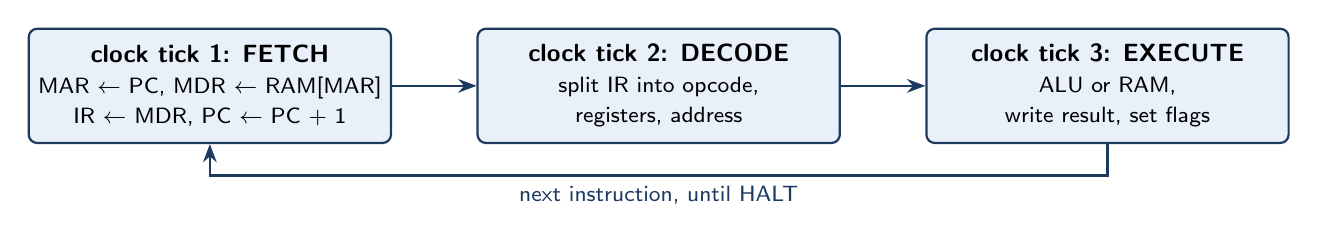
\begin{tikzpicture}[>=Stealth, font=\sffamily\small,
  st/.style={draw=frame, thick, fill=boxc, rounded corners=3pt, minimum width=4.6cm, minimum height=1.45cm, align=center}]
\node[st] (f) at (0,0) {\textbf{clock tick 1: FETCH}\\\footnotesize MAR $\leftarrow$ PC, MDR $\leftarrow$ RAM[MAR]\\\footnotesize IR $\leftarrow$ MDR, PC $\leftarrow$ PC + 1};
\node[st] (d) at (5.7,0) {\textbf{clock tick 2: DECODE}\\\footnotesize split IR into opcode,\\\footnotesize registers, address};
\node[st] (e) at (11.4,0) {\textbf{clock tick 3: EXECUTE}\\\footnotesize ALU or RAM,\\\footnotesize write result, set flags};
\draw[->, thick, frame] (f) -- (d);
\draw[->, thick, frame] (d) -- (e);
\draw[->, thick, frame] (e.south) -- ++(0,-0.4) -| node[pos=0.25, below, font=\footnotesize\sffamily]{next instruction, until HALT} (f.south);
\end{tikzpicture}
\caption{Fetch, decode, execute: one clock tick each}
\label{fig:cycle}
\end{figurehere}

% =====================================================================
\clearpage
\section{The CPU in Our C Program}\label{sec:struct}

\begin{figurehere}
\captionof{figure}{The CPU as a C struct (\texttt{src/cpu.h})}
\label{fig:struct}
\begin{lstlisting}[style=csrc]
/* The whole computer. */
typedef struct {
    /* special purpose registers */
    Register pc, ir, mar, mdr;
    Flags flags;
    /* general purpose registers R0..R7 */
    RegisterFile regs;
    /* the rest of the CPU */
    ALU alu;
    Clock clock;
    /* outside the CPU, connected by the system bus */
    SystemBus bus;
    Memory memory;
    OutputPort out_port;

    int halted;
    int steps;
} CPU;
\end{lstlisting}

\end{figurehere}

\begin{tablehere}
\caption{Each CPU part and its C code}
\label{tab:parts}
\small
\setlength{\tabcolsep}{4pt}
\begin{tabularx}{\textwidth}{@{}l l X l@{}}
\toprule
Part & Size & Job & In our C code \\
\midrule
PC, IR, MAR, MDR & 8 / 16 bits & special purpose registers & \texttt{Register} \\
FLAGS & 4 bits & Z, N, C, V & \texttt{Flags} \\
R0 to R7 & 8 $\times$ 16 bits & general purpose registers & \texttt{RegisterFile} \\
ALU & 16 bits & ADD, SUB, MUL, AND, OR, sets FLAGS & \texttt{ALU}, \texttt{alu\_compute()} \\
Control unit & & decode IR, test branch conditions & \texttt{control\_decode()} \\
Clock & & one tick per fetch, decode, execute & \texttt{Clock}, \texttt{clock\_tick()} \\
System bus & 8 + 16 bits & address, data and control bus & \texttt{SystemBus} \\
RAM & 256 $\times$ 16 bits & program and data & \texttt{Memory} \\
Output port & & prints what \texttt{OUT} sends & \texttt{OutputPort} \\
Fetch, decode, execute & & runs one instruction & \texttt{cpu\_step()} \\
\bottomrule
\end{tabularx}
\end{tablehere}

% =====================================================================
\clearpage
\section{Instruction Set}\label{sec:isa}

\begin{figurehere}
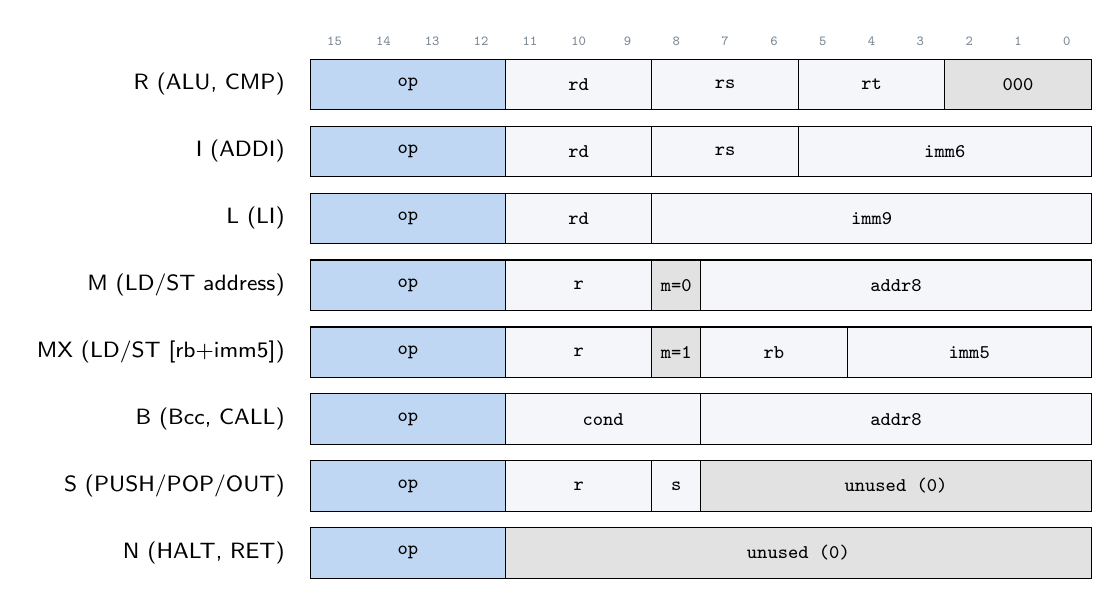
\begin{tikzpicture}
\node[font=\tiny\ttfamily, text=dim] at (9.610, -0.3) {0};
\node[font=\tiny\ttfamily, text=dim] at (8.990, -0.3) {1};
\node[font=\tiny\ttfamily, text=dim] at (8.370, -0.3) {2};
\node[font=\tiny\ttfamily, text=dim] at (7.750, -0.3) {3};
\node[font=\tiny\ttfamily, text=dim] at (7.130, -0.3) {4};
\node[font=\tiny\ttfamily, text=dim] at (6.510, -0.3) {5};
\node[font=\tiny\ttfamily, text=dim] at (5.890, -0.3) {6};
\node[font=\tiny\ttfamily, text=dim] at (5.270, -0.3) {7};
\node[font=\tiny\ttfamily, text=dim] at (4.650, -0.3) {8};
\node[font=\tiny\ttfamily, text=dim] at (4.030, -0.3) {9};
\node[font=\tiny\ttfamily, text=dim] at (3.410, -0.3) {10};
\node[font=\tiny\ttfamily, text=dim] at (2.790, -0.3) {11};
\node[font=\tiny\ttfamily, text=dim] at (2.170, -0.3) {12};
\node[font=\tiny\ttfamily, text=dim] at (1.550, -0.3) {13};
\node[font=\tiny\ttfamily, text=dim] at (0.930, -0.3) {14};
\node[font=\tiny\ttfamily, text=dim] at (0.310, -0.3) {15};
\node[anchor=east, font=\footnotesize\sffamily] at (-0.2, -0.85) {R (ALU, CMP)};
\draw[fill=opc] (0.000,-1.17) rectangle (2.480,-0.53);
\node[font=\scriptsize\ttfamily] at (1.240,-0.85) {op};
\draw[fill=fld] (2.480,-1.17) rectangle (4.340,-0.53);
\node[font=\scriptsize\ttfamily] at (3.410,-0.85) {rd};
\draw[fill=fld] (4.340,-1.17) rectangle (6.200,-0.53);
\node[font=\scriptsize\ttfamily] at (5.270,-0.85) {rs};
\draw[fill=fld] (6.200,-1.17) rectangle (8.060,-0.53);
\node[font=\scriptsize\ttfamily] at (7.130,-0.85) {rt};
\draw[fill=fixed] (8.060,-1.17) rectangle (9.920,-0.53);
\node[font=\scriptsize\ttfamily] at (8.990,-0.85) {000};
\node[anchor=east, font=\footnotesize\sffamily] at (-0.2, -1.70) {I (ADDI)};
\draw[fill=opc] (0.000,-2.02) rectangle (2.480,-1.38);
\node[font=\scriptsize\ttfamily] at (1.240,-1.70) {op};
\draw[fill=fld] (2.480,-2.02) rectangle (4.340,-1.38);
\node[font=\scriptsize\ttfamily] at (3.410,-1.70) {rd};
\draw[fill=fld] (4.340,-2.02) rectangle (6.200,-1.38);
\node[font=\scriptsize\ttfamily] at (5.270,-1.70) {rs};
\draw[fill=fld] (6.200,-2.02) rectangle (9.920,-1.38);
\node[font=\scriptsize\ttfamily] at (8.060,-1.70) {imm6};
\node[anchor=east, font=\footnotesize\sffamily] at (-0.2, -2.55) {L (LI)};
\draw[fill=opc] (0.000,-2.87) rectangle (2.480,-2.23);
\node[font=\scriptsize\ttfamily] at (1.240,-2.55) {op};
\draw[fill=fld] (2.480,-2.87) rectangle (4.340,-2.23);
\node[font=\scriptsize\ttfamily] at (3.410,-2.55) {rd};
\draw[fill=fld] (4.340,-2.87) rectangle (9.920,-2.23);
\node[font=\scriptsize\ttfamily] at (7.130,-2.55) {imm9};
\node[anchor=east, font=\footnotesize\sffamily] at (-0.2, -3.40) {M (LD/ST address)};
\draw[fill=opc] (0.000,-3.72) rectangle (2.480,-3.08);
\node[font=\scriptsize\ttfamily] at (1.240,-3.40) {op};
\draw[fill=fld] (2.480,-3.72) rectangle (4.340,-3.08);
\node[font=\scriptsize\ttfamily] at (3.410,-3.40) {r};
\draw[fill=fixed] (4.340,-3.72) rectangle (4.960,-3.08);
\node[font=\scriptsize\ttfamily] at (4.650,-3.40) {m=0};
\draw[fill=fld] (4.960,-3.72) rectangle (9.920,-3.08);
\node[font=\scriptsize\ttfamily] at (7.440,-3.40) {addr8};
\node[anchor=east, font=\footnotesize\sffamily] at (-0.2, -4.25) {MX (LD/ST [rb+imm5])};
\draw[fill=opc] (0.000,-4.57) rectangle (2.480,-3.93);
\node[font=\scriptsize\ttfamily] at (1.240,-4.25) {op};
\draw[fill=fld] (2.480,-4.57) rectangle (4.340,-3.93);
\node[font=\scriptsize\ttfamily] at (3.410,-4.25) {r};
\draw[fill=fixed] (4.340,-4.57) rectangle (4.960,-3.93);
\node[font=\scriptsize\ttfamily] at (4.650,-4.25) {m=1};
\draw[fill=fld] (4.960,-4.57) rectangle (6.820,-3.93);
\node[font=\scriptsize\ttfamily] at (5.890,-4.25) {rb};
\draw[fill=fld] (6.820,-4.57) rectangle (9.920,-3.93);
\node[font=\scriptsize\ttfamily] at (8.370,-4.25) {imm5};
\node[anchor=east, font=\footnotesize\sffamily] at (-0.2, -5.10) {B (Bcc, CALL)};
\draw[fill=opc] (0.000,-5.42) rectangle (2.480,-4.78);
\node[font=\scriptsize\ttfamily] at (1.240,-5.10) {op};
\draw[fill=fld] (2.480,-5.42) rectangle (4.960,-4.78);
\node[font=\scriptsize\ttfamily] at (3.720,-5.10) {cond};
\draw[fill=fld] (4.960,-5.42) rectangle (9.920,-4.78);
\node[font=\scriptsize\ttfamily] at (7.440,-5.10) {addr8};
\node[anchor=east, font=\footnotesize\sffamily] at (-0.2, -5.95) {S (PUSH/POP/OUT)};
\draw[fill=opc] (0.000,-6.27) rectangle (2.480,-5.63);
\node[font=\scriptsize\ttfamily] at (1.240,-5.95) {op};
\draw[fill=fld] (2.480,-6.27) rectangle (4.340,-5.63);
\node[font=\scriptsize\ttfamily] at (3.410,-5.95) {r};
\draw[fill=fld] (4.340,-6.27) rectangle (4.960,-5.63);
\node[font=\scriptsize\ttfamily] at (4.650,-5.95) {s};
\draw[fill=fixed] (4.960,-6.27) rectangle (9.920,-5.63);
\node[font=\scriptsize\ttfamily] at (7.440,-5.95) {unused (0)};
\node[anchor=east, font=\footnotesize\sffamily] at (-0.2, -6.80) {N (HALT, RET)};
\draw[fill=opc] (0.000,-7.12) rectangle (2.480,-6.48);
\node[font=\scriptsize\ttfamily] at (1.240,-6.80) {op};
\draw[fill=fixed] (2.480,-7.12) rectangle (9.920,-6.48);
\node[font=\scriptsize\ttfamily] at (6.200,-6.80) {unused (0)};

\end{tikzpicture}
\caption{Instruction formats, bit 15 on the left. Blue = opcode, grey = fixed bits.}
\label{fig:formats}
\end{figurehere}

\begin{tablehere}
\caption{Instruction table: every instruction and its binary code. \texttt{d s t r b} = register bits, \texttt{i} = number, \texttt{a} = address, \texttt{c} = condition.}
\label{tab:encoding}
\small
\setlength{\tabcolsep}{4pt}
\begin{tabular}{@{}llc l l l@{}}
\toprule
Opcode & Name & Fmt & Binary code [15:0] & What it does & Flags\\
\midrule
\rawinput generated/isa_table.tex
\bottomrule
\end{tabular}
\end{tablehere}

\begin{tablehere}
\caption{Branch conditions (\texttt{cccc} in Bcc)}
\label{tab:cond}
\small
\begin{tabular}{@{}llll@{}}
\toprule
cccc & Name & Jumps when & C op\\
\midrule
\rawinput generated/cond_table.tex
\bottomrule
\end{tabular}
\end{tablehere}

% =====================================================================
\clearpage
\section{How to Run}\label{sec:run}

\begin{tablehere}
\caption{Getting the code and running it. Needs \texttt{git}, a C compiler and \texttt{make}.}
\label{tab:getcode}
\small
\begin{tabular}{@{}cll@{}}
\toprule
Step & Command & What it does \\
\midrule
1 & {\footnotesize\texttt{git clone https://github.com/vineetkia/CMPE-220-CPU-Simulation-Project.git}} & downloads the code \\
2 & \texttt{cd CMPE-220-CPU-Simulation-Project} & goes into the project folder \\
3 & \texttt{make} & builds the \texttt{spartan} program \\
4 & \texttt{./spartan run add} & runs program 1 \\
5 & \texttt{./spartan run multiply} & runs program 2 \\
\bottomrule
\end{tabular}
\end{tablehere}

\begin{tablehere}
\caption{All commands}
\label{tab:commands}
\small
\begin{tabular}{@{}ll@{}}
\toprule
Command & What you get \\
\midrule
\texttt{./spartan run add} & program 1, every instruction \\
\texttt{./spartan run multiply} & program 2, every instruction \\
\texttt{./spartan run add -{}-quiet} & just the answer \\
\texttt{./spartan isa} & the instruction table \\
\texttt{make test} & the tests \\
\texttt{make report} & this PDF, made again from the simulator \\
\bottomrule
\end{tabular}
\end{tablehere}

\begin{figurehere}
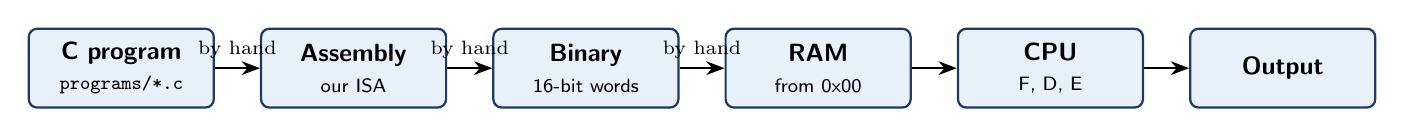
\begin{tikzpicture}[>=Stealth, font=\sffamily\small,
  st/.style={draw=frame, thick, fill=boxc, rounded corners=3pt, minimum width=2.35cm, minimum height=1.0cm, align=center}]
\node[st] (c) at (0,0) {\textbf{C program}\\\scriptsize \texttt{programs/*.c}};
\node[st] (a) at (2.95,0) {\textbf{Assembly}\\\scriptsize our ISA};
\node[st] (b) at (5.9,0) {\textbf{Binary}\\\scriptsize 16-bit words};
\node[st] (r) at (8.85,0) {\textbf{RAM}\\\scriptsize from 0x00};
\node[st] (p) at (11.8,0) {\textbf{CPU}\\\scriptsize F, D, E};
\node[st] (o) at (14.75,0) {\textbf{Output}};
\draw[->, thick] (c) -- node[above, font=\scriptsize]{by hand} (a);
\draw[->, thick] (a) -- node[above, font=\scriptsize]{by hand} (b);
\draw[->, thick] (b) -- node[above, font=\scriptsize]{by hand} (r);
\draw[->, thick] (r) -- (p);
\draw[->, thick] (p) -- (o);
\end{tikzpicture}
\caption{Our process for each program. The binary is in \texttt{src/programs.c}.}
\label{fig:process}
\end{figurehere}

% =====================================================================
\clearpage
\section{Program 1: Add Two Numbers}\label{sec:add}

\begin{figurehere}
\captionof{figure}{\texttt{programs/add.c}}
\label{fig:addc}
\begin{lstlisting}[style=csrc]
#include <stdio.h>

int a = 5;
int b = 7;
int c;

int main(void)
{
    c = a + b;
    printf("%d\n", c);
    return 0;
}
\end{lstlisting}

\end{figurehere}

\begin{tablehere}
\caption{add.c translated by hand: C line, our assembly, our binary. Shaded rows are data.}
\label{tab:addtrans}
\small
\begin{tabular}{@{}lllll@{}}
\toprule
Addr & C line & Assembly & Binary (fields) & Hex\\
\midrule
\rawinput generated/add_translate.tex
\bottomrule
\end{tabular}
\end{tablehere}

\begin{tablehere}
\caption{RAM after we put the binary in by hand. PC = 00, so the program starts at 00.}
\label{tab:addram}
\small
\begin{tabular}{@{}>{\ttfamily}l >{\ttfamily}l >{\ttfamily}l >{\ttfamily}l >{\ttfamily}l@{}}
\toprule
\rmfamily Addr & \rmfamily Binary & \rmfamily Hex & \rmfamily ASCII & \rmfamily Content\\
\midrule
\rawinput generated/add_ram.tex
\bottomrule
\end{tabular}
\end{tablehere}

\clearpage
\subsection{Program 1: fetch, decode, execute}
\captionof{figure}{add.c: CPU and RAM after every instruction (\addSteps{} instructions, \addTicks{} clock ticks)}
\label{fig:addtrace}
\legend
\noindent\begin{tcolorbox}[stepbox, title={Instruction 1 \hfill ticks 1 to 3 \quad LD R1, a}]
\textcolor{dim}{tick 1} \textbf{F} MAR$\leftarrow$00, MDR$\leftarrow$RAM[00]=8206, IR$\leftarrow$MDR, PC$\leftarrow$01\\
\textcolor{dim}{tick 2} \textbf{D} 1000 001 0 00000110 = LD R1, a\\
\textcolor{dim}{tick 3} \textbf{E} R1 $\leftarrow$ M[0x06] (a) = 5\\[2pt]
\textcolor{dim}{special purpose registers (binary [ASCII])}\\
PC~~00000001 [.] \hfill IR~~1000001000000110 [..]\\
MAR 00000110 [.] \hfill MDR 0000000000000101 [..]\\
FLAGS Z=0 N=0 C=0 V=0\\[2pt]
\textcolor{dim}{general purpose registers (binary, decimal [ASCII])}\\
R0 0000000000000000 0 [..] \hfill R4 0000000000000000 0 [..]\\
\textcolor{wrt}{\textbf{R1 0000000000000101 5 [..]}} \hfill R5 0000000000000000 0 [..]\\
R2 0000000000000000 0 [..] \hfill R6 0000000000000000 0 [..]\\
R3 0000000000000000 0 [..] \hfill SP 0000000000000000 0 [..]\\
\textcolor{dim}{ALU not used}\\[2pt]
{\setlength{\tabcolsep}{2pt}\begin{tabular}{@{}lllll@{}}
\textcolor{dim}{addr} & \textcolor{dim}{binary} & \textcolor{dim}{hex} & \textcolor{dim}{ascii} & \textcolor{dim}{content}\\
00 & 1000001000000110 & 8206 & .. & LD R1, a\\
\rowcolor{pcc}01 & 1000010000000111 & 8407 & .. & LD R2, b\\
02 & 0001011001010000 & 1650 & .P & ADD R3, R1, R2\\
03 & 1001011000001000 & 9608 & .. & ST R3, c\\
04 & 1111011000000000 & F600 & .. & OUT R3\\
05 & 0000000000000000 & 0000 & .. & HALT\\
\rowcolor{datac}06 & 0000000000000101 & 0005 & .. & a = 5\\
\rowcolor{datac}07 & 0000000000000111 & 0007 & .. & b = 7\\
\rowcolor{datac}08 & 0000000000000000 & 0000 & .. & c = 0\\
\end{tabular}}
\end{tcolorbox}\hfill\begin{tcolorbox}[stepbox, title={Instruction 2 \hfill ticks 4 to 6 \quad LD R2, b}]
\textcolor{dim}{tick 4} \textbf{F} MAR$\leftarrow$01, MDR$\leftarrow$RAM[01]=8407, IR$\leftarrow$MDR, PC$\leftarrow$02\\
\textcolor{dim}{tick 5} \textbf{D} 1000 010 0 00000111 = LD R2, b\\
\textcolor{dim}{tick 6} \textbf{E} R2 $\leftarrow$ M[0x07] (b) = 7\\[2pt]
\textcolor{dim}{special purpose registers (binary [ASCII])}\\
PC~~00000010 [.] \hfill IR~~1000010000000111 [..]\\
MAR 00000111 [.] \hfill MDR 0000000000000111 [..]\\
FLAGS Z=0 N=0 C=0 V=0\\[2pt]
\textcolor{dim}{general purpose registers (binary, decimal [ASCII])}\\
R0 0000000000000000 0 [..] \hfill R4 0000000000000000 0 [..]\\
R1 0000000000000101 5 [..] \hfill R5 0000000000000000 0 [..]\\
\textcolor{wrt}{\textbf{R2 0000000000000111 7 [..]}} \hfill R6 0000000000000000 0 [..]\\
R3 0000000000000000 0 [..] \hfill SP 0000000000000000 0 [..]\\
\textcolor{dim}{ALU not used}\\[2pt]
{\setlength{\tabcolsep}{2pt}\begin{tabular}{@{}lllll@{}}
\textcolor{dim}{addr} & \textcolor{dim}{binary} & \textcolor{dim}{hex} & \textcolor{dim}{ascii} & \textcolor{dim}{content}\\
00 & 1000001000000110 & 8206 & .. & LD R1, a\\
01 & 1000010000000111 & 8407 & .. & LD R2, b\\
\rowcolor{pcc}02 & 0001011001010000 & 1650 & .P & ADD R3, R1, R2\\
03 & 1001011000001000 & 9608 & .. & ST R3, c\\
04 & 1111011000000000 & F600 & .. & OUT R3\\
05 & 0000000000000000 & 0000 & .. & HALT\\
\rowcolor{datac}06 & 0000000000000101 & 0005 & .. & a = 5\\
\rowcolor{datac}07 & 0000000000000111 & 0007 & .. & b = 7\\
\rowcolor{datac}08 & 0000000000000000 & 0000 & .. & c = 0\\
\end{tabular}}
\end{tcolorbox}\par\vspace{3pt}
\noindent\begin{tcolorbox}[stepbox, title={Instruction 3 \hfill ticks 7 to 9 \quad ADD R3, R1, R2}]
\textcolor{dim}{tick 7} \textbf{F} MAR$\leftarrow$02, MDR$\leftarrow$RAM[02]=1650, IR$\leftarrow$MDR, PC$\leftarrow$03\\
\textcolor{dim}{tick 8} \textbf{D} 0001 011 001 010 000 = ADD R3, R1, R2\\
\textcolor{dim}{tick 9} \textbf{E} R3 $\leftarrow$ 5 + 7 = 12\\[2pt]
\textcolor{dim}{special purpose registers (binary [ASCII])}\\
PC~~00000011 [.] \hfill IR~~0001011001010000 [.P]\\
MAR 00000010 [.] \hfill MDR 0001011001010000 [.P]\\
FLAGS Z=0 N=0 C=0 V=0\\[2pt]
\textcolor{dim}{general purpose registers (binary, decimal [ASCII])}\\
R0 0000000000000000 0 [..] \hfill R4 0000000000000000 0 [..]\\
R1 0000000000000101 5 [..] \hfill R5 0000000000000000 0 [..]\\
R2 0000000000000111 7 [..] \hfill R6 0000000000000000 0 [..]\\
\textcolor{wrt}{\textbf{R3 0000000000001100 12 [..]}} \hfill SP 0000000000000000 0 [..]\\
\textcolor{dim}{ALU} ADD: 5 + 7 = 12 [..] \hfill 0000000000001100\\[2pt]
{\setlength{\tabcolsep}{2pt}\begin{tabular}{@{}lllll@{}}
\textcolor{dim}{addr} & \textcolor{dim}{binary} & \textcolor{dim}{hex} & \textcolor{dim}{ascii} & \textcolor{dim}{content}\\
00 & 1000001000000110 & 8206 & .. & LD R1, a\\
01 & 1000010000000111 & 8407 & .. & LD R2, b\\
02 & 0001011001010000 & 1650 & .P & ADD R3, R1, R2\\
\rowcolor{pcc}03 & 1001011000001000 & 9608 & .. & ST R3, c\\
04 & 1111011000000000 & F600 & .. & OUT R3\\
05 & 0000000000000000 & 0000 & .. & HALT\\
\rowcolor{datac}06 & 0000000000000101 & 0005 & .. & a = 5\\
\rowcolor{datac}07 & 0000000000000111 & 0007 & .. & b = 7\\
\rowcolor{datac}08 & 0000000000000000 & 0000 & .. & c = 0\\
\end{tabular}}
\end{tcolorbox}\hfill\begin{tcolorbox}[stepbox, title={Instruction 4 \hfill ticks 10 to 12 \quad ST R3, c}]
\textcolor{dim}{tick 10} \textbf{F} MAR$\leftarrow$03, MDR$\leftarrow$RAM[03]=9608, IR$\leftarrow$MDR, PC$\leftarrow$04\\
\textcolor{dim}{tick 11} \textbf{D} 1001 011 0 00001000 = ST R3, c\\
\textcolor{dim}{tick 12} \textbf{E} M[0x08] (c) $\leftarrow$ R3 = 12\\[2pt]
\textcolor{dim}{special purpose registers (binary [ASCII])}\\
PC~~00000100 [.] \hfill IR~~1001011000001000 [..]\\
MAR 00001000 [.] \hfill MDR 0000000000001100 [..]\\
FLAGS Z=0 N=0 C=0 V=0\\[2pt]
\textcolor{dim}{general purpose registers (binary, decimal [ASCII])}\\
R0 0000000000000000 0 [..] \hfill R4 0000000000000000 0 [..]\\
R1 0000000000000101 5 [..] \hfill R5 0000000000000000 0 [..]\\
R2 0000000000000111 7 [..] \hfill R6 0000000000000000 0 [..]\\
R3 0000000000001100 12 [..] \hfill SP 0000000000000000 0 [..]\\
\textcolor{dim}{ALU not used}\\[2pt]
{\setlength{\tabcolsep}{2pt}\begin{tabular}{@{}lllll@{}}
\textcolor{dim}{addr} & \textcolor{dim}{binary} & \textcolor{dim}{hex} & \textcolor{dim}{ascii} & \textcolor{dim}{content}\\
00 & 1000001000000110 & 8206 & .. & LD R1, a\\
01 & 1000010000000111 & 8407 & .. & LD R2, b\\
02 & 0001011001010000 & 1650 & .P & ADD R3, R1, R2\\
03 & 1001011000001000 & 9608 & .. & ST R3, c\\
\rowcolor{pcc}04 & 1111011000000000 & F600 & .. & OUT R3\\
05 & 0000000000000000 & 0000 & .. & HALT\\
\rowcolor{datac}06 & 0000000000000101 & 0005 & .. & a = 5\\
\rowcolor{datac}07 & 0000000000000111 & 0007 & .. & b = 7\\
\rowcolor{wrt}\textcolor{white}{\textbf{08}} & \textcolor{white}{\textbf{0000000000001100}} & \textcolor{white}{\textbf{000C}} & \textcolor{white}{\textbf{..}} & \textcolor{white}{\textbf{c = 12}}\\
\end{tabular}}
\end{tcolorbox}\par\vspace{3pt}
\noindent\begin{tcolorbox}[stepbox, title={Instruction 5 \hfill ticks 13 to 15 \quad OUT R3}]
\textcolor{dim}{tick 13} \textbf{F} MAR$\leftarrow$04, MDR$\leftarrow$RAM[04]=F600, IR$\leftarrow$MDR, PC$\leftarrow$05\\
\textcolor{dim}{tick 14} \textbf{D} 1111 011 0 00000000 = OUT R3\\
\textcolor{dim}{tick 15} \textbf{E} output R3 = 12 \hfill \colorbox{outc}{\textbf{OUTPUT: 12}}\\[2pt]
\textcolor{dim}{special purpose registers (binary [ASCII])}\\
PC~~00000101 [.] \hfill IR~~1111011000000000 [..]\\
MAR 00000100 [.] \hfill MDR 1111011000000000 [..]\\
FLAGS Z=0 N=0 C=0 V=0\\[2pt]
\textcolor{dim}{general purpose registers (binary, decimal [ASCII])}\\
R0 0000000000000000 0 [..] \hfill R4 0000000000000000 0 [..]\\
R1 0000000000000101 5 [..] \hfill R5 0000000000000000 0 [..]\\
R2 0000000000000111 7 [..] \hfill R6 0000000000000000 0 [..]\\
R3 0000000000001100 12 [..] \hfill SP 0000000000000000 0 [..]\\
\textcolor{dim}{ALU not used}\\[2pt]
{\setlength{\tabcolsep}{2pt}\begin{tabular}{@{}lllll@{}}
\textcolor{dim}{addr} & \textcolor{dim}{binary} & \textcolor{dim}{hex} & \textcolor{dim}{ascii} & \textcolor{dim}{content}\\
00 & 1000001000000110 & 8206 & .. & LD R1, a\\
01 & 1000010000000111 & 8407 & .. & LD R2, b\\
02 & 0001011001010000 & 1650 & .P & ADD R3, R1, R2\\
03 & 1001011000001000 & 9608 & .. & ST R3, c\\
04 & 1111011000000000 & F600 & .. & OUT R3\\
\rowcolor{pcc}05 & 0000000000000000 & 0000 & .. & HALT\\
\rowcolor{datac}06 & 0000000000000101 & 0005 & .. & a = 5\\
\rowcolor{datac}07 & 0000000000000111 & 0007 & .. & b = 7\\
\rowcolor{datac}08 & 0000000000001100 & 000C & .. & c = 12\\
\end{tabular}}
\end{tcolorbox}\hfill\begin{tcolorbox}[stepbox, title={Instruction 6 \hfill ticks 16 to 18 \quad HALT}]
\textcolor{dim}{tick 16} \textbf{F} MAR$\leftarrow$05, MDR$\leftarrow$RAM[05]=0000, IR$\leftarrow$MDR, PC$\leftarrow$06\\
\textcolor{dim}{tick 17} \textbf{D} 0000 000000000000 = HALT\\
\textcolor{dim}{tick 18} \textbf{E} processor halted\\[2pt]
\textcolor{dim}{special purpose registers (binary [ASCII])}\\
PC~~00000110 [.] \hfill IR~~0000000000000000 [..]\\
MAR 00000101 [.] \hfill MDR 0000000000000000 [..]\\
FLAGS Z=0 N=0 C=0 V=0\\[2pt]
\textcolor{dim}{general purpose registers (binary, decimal [ASCII])}\\
R0 0000000000000000 0 [..] \hfill R4 0000000000000000 0 [..]\\
R1 0000000000000101 5 [..] \hfill R5 0000000000000000 0 [..]\\
R2 0000000000000111 7 [..] \hfill R6 0000000000000000 0 [..]\\
R3 0000000000001100 12 [..] \hfill SP 0000000000000000 0 [..]\\
\textcolor{dim}{ALU not used}\\[2pt]
{\setlength{\tabcolsep}{2pt}\begin{tabular}{@{}lllll@{}}
\textcolor{dim}{addr} & \textcolor{dim}{binary} & \textcolor{dim}{hex} & \textcolor{dim}{ascii} & \textcolor{dim}{content}\\
00 & 1000001000000110 & 8206 & .. & LD R1, a\\
01 & 1000010000000111 & 8407 & .. & LD R2, b\\
02 & 0001011001010000 & 1650 & .P & ADD R3, R1, R2\\
03 & 1001011000001000 & 9608 & .. & ST R3, c\\
04 & 1111011000000000 & F600 & .. & OUT R3\\
05 & 0000000000000000 & 0000 & .. & HALT\\
\rowcolor{datac}06 & 0000000000000101 & 0005 & .. & a = 5\\
\rowcolor{datac}07 & 0000000000000111 & 0007 & .. & b = 7\\
\rowcolor{datac}08 & 0000000000001100 & 000C & .. & c = 12\\
\end{tabular}}
\end{tcolorbox}\par\vspace{3pt}


% =====================================================================
\clearpage
\section{Program 2: Multiply Two Numbers Using Only ADD}\label{sec:mul}

\begin{figurehere}
\captionof{figure}{\texttt{programs/multiply.c}}
\label{fig:mulc}
\begin{lstlisting}[style=csrc]
#include <stdio.h>

int a = 5;
int b = 3;
int result = 0;

int main(void)
{
    while (b > 0) {
        result = result + a;
        b = b - 1;
    }
    printf("%d\n", result);
    return 0;
}
\end{lstlisting}

\end{figurehere}

\begin{tablehere}
\caption{multiply.c translated by hand: C line, our assembly, our binary. Shaded rows are data.}
\label{tab:multrans}
\small
\begin{tabular}{@{}lllll@{}}
\toprule
Addr & C line & Assembly & Binary (fields) & Hex\\
\midrule
\rawinput generated/mul_translate.tex
\bottomrule
\end{tabular}
\end{tablehere}

\begin{tablehere}
\caption{RAM after we put the binary in by hand. PC = 00, so the program starts at 00.}
\label{tab:mulram}
\small
\begin{tabular}{@{}>{\ttfamily}l >{\ttfamily}l >{\ttfamily}l >{\ttfamily}l >{\ttfamily}l@{}}
\toprule
\rmfamily Addr & \rmfamily Binary & \rmfamily Hex & \rmfamily ASCII & \rmfamily Content\\
\midrule
\rawinput generated/mul_ram.tex
\bottomrule
\end{tabular}
\end{tablehere}

\clearpage
\subsection{Program 2: fetch, decode, execute}
\captionof{figure}{multiply.c: CPU and RAM after every instruction (\mulSteps{} instructions, \mulTicks{} clock ticks)}
\label{fig:multrace}
\legend
\noindent\begin{tcolorbox}[stepbox, title={Instruction 1 \hfill ticks 1 to 3 \quad LD R1, a}]
\textcolor{dim}{tick 1} \textbf{F} MAR$\leftarrow$00, MDR$\leftarrow$RAM[00]=820C, IR$\leftarrow$MDR, PC$\leftarrow$01\\
\textcolor{dim}{tick 2} \textbf{D} 1000 001 0 00001100 = LD R1, a\\
\textcolor{dim}{tick 3} \textbf{E} R1 $\leftarrow$ M[0x0C] (a) = 5\\[2pt]
\textcolor{dim}{special purpose registers (binary [ASCII])}\\
PC~~00000001 [.] \hfill IR~~1000001000001100 [..]\\
MAR 00001100 [.] \hfill MDR 0000000000000101 [..]\\
FLAGS Z=0 N=0 C=0 V=0\\[2pt]
\textcolor{dim}{general purpose registers (binary, decimal [ASCII])}\\
R0 0000000000000000 0 [..] \hfill R4 0000000000000000 0 [..]\\
\textcolor{wrt}{\textbf{R1 0000000000000101 5 [..]}} \hfill R5 0000000000000000 0 [..]\\
R2 0000000000000000 0 [..] \hfill R6 0000000000000000 0 [..]\\
R3 0000000000000000 0 [..] \hfill SP 0000000000000000 0 [..]\\
\textcolor{dim}{ALU not used}\\[2pt]
{\setlength{\tabcolsep}{2pt}\begin{tabular}{@{}lllll@{}}
\textcolor{dim}{addr} & \textcolor{dim}{binary} & \textcolor{dim}{hex} & \textcolor{dim}{ascii} & \textcolor{dim}{content}\\
00 & 1000001000001100 & 820C & .. & LD R1, a\\
\rowcolor{pcc}01 & 1000010000001101 & 840D & .. & LD R2, b\\
02 & 0111011000000000 & 7600 & v. & LI R3, 0\\
03 & 1010000010000000 & A080 & .. & CMP R2, R0\\
04 & 1011011000001010 & B60A & .. & BLE done\\
05 & 0001011011001000 & 16C8 & .. & ADD R3, R3, R1\\
06 & 1001011000001110 & 960E & .. & ST R3, result\\
07 & 0110010010111111 & 64BF & d. & ADDI R2, R2, -1\\
08 & 1001010000001101 & 940D & .. & ST R2, b\\
09 & 1011000000000011 & B003 & .. & JMP loop\\
0A & 1111011000000000 & F600 & .. & OUT R3\\
0B & 0000000000000000 & 0000 & .. & HALT\\
\rowcolor{datac}0C & 0000000000000101 & 0005 & .. & a = 5\\
\rowcolor{datac}0D & 0000000000000011 & 0003 & .. & b = 3\\
\rowcolor{datac}0E & 0000000000000000 & 0000 & .. & result = 0\\
\end{tabular}}
\end{tcolorbox}\hfill\begin{tcolorbox}[stepbox, title={Instruction 2 \hfill ticks 4 to 6 \quad LD R2, b}]
\textcolor{dim}{tick 4} \textbf{F} MAR$\leftarrow$01, MDR$\leftarrow$RAM[01]=840D, IR$\leftarrow$MDR, PC$\leftarrow$02\\
\textcolor{dim}{tick 5} \textbf{D} 1000 010 0 00001101 = LD R2, b\\
\textcolor{dim}{tick 6} \textbf{E} R2 $\leftarrow$ M[0x0D] (b) = 3\\[2pt]
\textcolor{dim}{special purpose registers (binary [ASCII])}\\
PC~~00000010 [.] \hfill IR~~1000010000001101 [..]\\
MAR 00001101 [.] \hfill MDR 0000000000000011 [..]\\
FLAGS Z=0 N=0 C=0 V=0\\[2pt]
\textcolor{dim}{general purpose registers (binary, decimal [ASCII])}\\
R0 0000000000000000 0 [..] \hfill R4 0000000000000000 0 [..]\\
R1 0000000000000101 5 [..] \hfill R5 0000000000000000 0 [..]\\
\textcolor{wrt}{\textbf{R2 0000000000000011 3 [..]}} \hfill R6 0000000000000000 0 [..]\\
R3 0000000000000000 0 [..] \hfill SP 0000000000000000 0 [..]\\
\textcolor{dim}{ALU not used}\\[2pt]
{\setlength{\tabcolsep}{2pt}\begin{tabular}{@{}lllll@{}}
\textcolor{dim}{addr} & \textcolor{dim}{binary} & \textcolor{dim}{hex} & \textcolor{dim}{ascii} & \textcolor{dim}{content}\\
00 & 1000001000001100 & 820C & .. & LD R1, a\\
01 & 1000010000001101 & 840D & .. & LD R2, b\\
\rowcolor{pcc}02 & 0111011000000000 & 7600 & v. & LI R3, 0\\
03 & 1010000010000000 & A080 & .. & CMP R2, R0\\
04 & 1011011000001010 & B60A & .. & BLE done\\
05 & 0001011011001000 & 16C8 & .. & ADD R3, R3, R1\\
06 & 1001011000001110 & 960E & .. & ST R3, result\\
07 & 0110010010111111 & 64BF & d. & ADDI R2, R2, -1\\
08 & 1001010000001101 & 940D & .. & ST R2, b\\
09 & 1011000000000011 & B003 & .. & JMP loop\\
0A & 1111011000000000 & F600 & .. & OUT R3\\
0B & 0000000000000000 & 0000 & .. & HALT\\
\rowcolor{datac}0C & 0000000000000101 & 0005 & .. & a = 5\\
\rowcolor{datac}0D & 0000000000000011 & 0003 & .. & b = 3\\
\rowcolor{datac}0E & 0000000000000000 & 0000 & .. & result = 0\\
\end{tabular}}
\end{tcolorbox}\par\vspace{3pt}
\noindent\begin{tcolorbox}[stepbox, title={Instruction 3 \hfill ticks 7 to 9 \quad LI R3, 0}]
\textcolor{dim}{tick 7} \textbf{F} MAR$\leftarrow$02, MDR$\leftarrow$RAM[02]=7600, IR$\leftarrow$MDR, PC$\leftarrow$03\\
\textcolor{dim}{tick 8} \textbf{D} 0111 011 000000000 = LI R3, 0\\
\textcolor{dim}{tick 9} \textbf{E} R3 $\leftarrow$ 0\\[2pt]
\textcolor{dim}{special purpose registers (binary [ASCII])}\\
PC~~00000011 [.] \hfill IR~~0111011000000000 [v.]\\
MAR 00000010 [.] \hfill MDR 0111011000000000 [v.]\\
FLAGS Z=0 N=0 C=0 V=0\\[2pt]
\textcolor{dim}{general purpose registers (binary, decimal [ASCII])}\\
R0 0000000000000000 0 [..] \hfill R4 0000000000000000 0 [..]\\
R1 0000000000000101 5 [..] \hfill R5 0000000000000000 0 [..]\\
R2 0000000000000011 3 [..] \hfill R6 0000000000000000 0 [..]\\
\textcolor{wrt}{\textbf{R3 0000000000000000 0 [..]}} \hfill SP 0000000000000000 0 [..]\\
\textcolor{dim}{ALU not used}\\[2pt]
{\setlength{\tabcolsep}{2pt}\begin{tabular}{@{}lllll@{}}
\textcolor{dim}{addr} & \textcolor{dim}{binary} & \textcolor{dim}{hex} & \textcolor{dim}{ascii} & \textcolor{dim}{content}\\
00 & 1000001000001100 & 820C & .. & LD R1, a\\
01 & 1000010000001101 & 840D & .. & LD R2, b\\
02 & 0111011000000000 & 7600 & v. & LI R3, 0\\
\rowcolor{pcc}03 & 1010000010000000 & A080 & .. & CMP R2, R0\\
04 & 1011011000001010 & B60A & .. & BLE done\\
05 & 0001011011001000 & 16C8 & .. & ADD R3, R3, R1\\
06 & 1001011000001110 & 960E & .. & ST R3, result\\
07 & 0110010010111111 & 64BF & d. & ADDI R2, R2, -1\\
08 & 1001010000001101 & 940D & .. & ST R2, b\\
09 & 1011000000000011 & B003 & .. & JMP loop\\
0A & 1111011000000000 & F600 & .. & OUT R3\\
0B & 0000000000000000 & 0000 & .. & HALT\\
\rowcolor{datac}0C & 0000000000000101 & 0005 & .. & a = 5\\
\rowcolor{datac}0D & 0000000000000011 & 0003 & .. & b = 3\\
\rowcolor{datac}0E & 0000000000000000 & 0000 & .. & result = 0\\
\end{tabular}}
\end{tcolorbox}\hfill\begin{tcolorbox}[stepbox, title={Instruction 4 \hfill ticks 10 to 12 \quad CMP R2, R0}]
\textcolor{dim}{tick 10} \textbf{F} MAR$\leftarrow$03, MDR$\leftarrow$RAM[03]=A080, IR$\leftarrow$MDR, PC$\leftarrow$04\\
\textcolor{dim}{tick 11} \textbf{D} 1010 000 010 000 000 = CMP R2, R0\\
\textcolor{dim}{tick 12} \textbf{E} compare 3 with 0, set flags\\[2pt]
\textcolor{dim}{special purpose registers (binary [ASCII])}\\
PC~~00000100 [.] \hfill IR~~1010000010000000 [..]\\
MAR 00000011 [.] \hfill MDR 1010000010000000 [..]\\
FLAGS Z=0 N=0 C=0 V=0\\[2pt]
\textcolor{dim}{general purpose registers (binary, decimal [ASCII])}\\
R0 0000000000000000 0 [..] \hfill R4 0000000000000000 0 [..]\\
R1 0000000000000101 5 [..] \hfill R5 0000000000000000 0 [..]\\
R2 0000000000000011 3 [..] \hfill R6 0000000000000000 0 [..]\\
R3 0000000000000000 0 [..] \hfill SP 0000000000000000 0 [..]\\
\textcolor{dim}{ALU} SUB: 3 $-$ 0 = 3 [..] \hfill 0000000000000011\\[2pt]
{\setlength{\tabcolsep}{2pt}\begin{tabular}{@{}lllll@{}}
\textcolor{dim}{addr} & \textcolor{dim}{binary} & \textcolor{dim}{hex} & \textcolor{dim}{ascii} & \textcolor{dim}{content}\\
00 & 1000001000001100 & 820C & .. & LD R1, a\\
01 & 1000010000001101 & 840D & .. & LD R2, b\\
02 & 0111011000000000 & 7600 & v. & LI R3, 0\\
03 & 1010000010000000 & A080 & .. & CMP R2, R0\\
\rowcolor{pcc}04 & 1011011000001010 & B60A & .. & BLE done\\
05 & 0001011011001000 & 16C8 & .. & ADD R3, R3, R1\\
06 & 1001011000001110 & 960E & .. & ST R3, result\\
07 & 0110010010111111 & 64BF & d. & ADDI R2, R2, -1\\
08 & 1001010000001101 & 940D & .. & ST R2, b\\
09 & 1011000000000011 & B003 & .. & JMP loop\\
0A & 1111011000000000 & F600 & .. & OUT R3\\
0B & 0000000000000000 & 0000 & .. & HALT\\
\rowcolor{datac}0C & 0000000000000101 & 0005 & .. & a = 5\\
\rowcolor{datac}0D & 0000000000000011 & 0003 & .. & b = 3\\
\rowcolor{datac}0E & 0000000000000000 & 0000 & .. & result = 0\\
\end{tabular}}
\end{tcolorbox}\par\vspace{3pt}
\noindent\begin{tcolorbox}[stepbox, title={Instruction 5 \hfill ticks 13 to 15 \quad BLE done}]
\textcolor{dim}{tick 13} \textbf{F} MAR$\leftarrow$04, MDR$\leftarrow$RAM[04]=B60A, IR$\leftarrow$MDR, PC$\leftarrow$05\\
\textcolor{dim}{tick 14} \textbf{D} 1011 0110 00001010 = BLE done\\
\textcolor{dim}{tick 15} \textbf{E} branch not taken\\[2pt]
\textcolor{dim}{special purpose registers (binary [ASCII])}\\
PC~~00000101 [.] \hfill IR~~1011011000001010 [..]\\
MAR 00000100 [.] \hfill MDR 1011011000001010 [..]\\
FLAGS Z=0 N=0 C=0 V=0\\[2pt]
\textcolor{dim}{general purpose registers (binary, decimal [ASCII])}\\
R0 0000000000000000 0 [..] \hfill R4 0000000000000000 0 [..]\\
R1 0000000000000101 5 [..] \hfill R5 0000000000000000 0 [..]\\
R2 0000000000000011 3 [..] \hfill R6 0000000000000000 0 [..]\\
R3 0000000000000000 0 [..] \hfill SP 0000000000000000 0 [..]\\
\textcolor{dim}{ALU not used}\\[2pt]
{\setlength{\tabcolsep}{2pt}\begin{tabular}{@{}lllll@{}}
\textcolor{dim}{addr} & \textcolor{dim}{binary} & \textcolor{dim}{hex} & \textcolor{dim}{ascii} & \textcolor{dim}{content}\\
00 & 1000001000001100 & 820C & .. & LD R1, a\\
01 & 1000010000001101 & 840D & .. & LD R2, b\\
02 & 0111011000000000 & 7600 & v. & LI R3, 0\\
03 & 1010000010000000 & A080 & .. & CMP R2, R0\\
04 & 1011011000001010 & B60A & .. & BLE done\\
\rowcolor{pcc}05 & 0001011011001000 & 16C8 & .. & ADD R3, R3, R1\\
06 & 1001011000001110 & 960E & .. & ST R3, result\\
07 & 0110010010111111 & 64BF & d. & ADDI R2, R2, -1\\
08 & 1001010000001101 & 940D & .. & ST R2, b\\
09 & 1011000000000011 & B003 & .. & JMP loop\\
0A & 1111011000000000 & F600 & .. & OUT R3\\
0B & 0000000000000000 & 0000 & .. & HALT\\
\rowcolor{datac}0C & 0000000000000101 & 0005 & .. & a = 5\\
\rowcolor{datac}0D & 0000000000000011 & 0003 & .. & b = 3\\
\rowcolor{datac}0E & 0000000000000000 & 0000 & .. & result = 0\\
\end{tabular}}
\end{tcolorbox}\hfill\begin{tcolorbox}[stepbox, title={Instruction 6 \hfill ticks 16 to 18 \quad ADD R3, R3, R1}]
\textcolor{dim}{tick 16} \textbf{F} MAR$\leftarrow$05, MDR$\leftarrow$RAM[05]=16C8, IR$\leftarrow$MDR, PC$\leftarrow$06\\
\textcolor{dim}{tick 17} \textbf{D} 0001 011 011 001 000 = ADD R3, R3, R1\\
\textcolor{dim}{tick 18} \textbf{E} R3 $\leftarrow$ 0 + 5 = 5\\[2pt]
\textcolor{dim}{special purpose registers (binary [ASCII])}\\
PC~~00000110 [.] \hfill IR~~0001011011001000 [..]\\
MAR 00000101 [.] \hfill MDR 0001011011001000 [..]\\
FLAGS Z=0 N=0 C=0 V=0\\[2pt]
\textcolor{dim}{general purpose registers (binary, decimal [ASCII])}\\
R0 0000000000000000 0 [..] \hfill R4 0000000000000000 0 [..]\\
R1 0000000000000101 5 [..] \hfill R5 0000000000000000 0 [..]\\
R2 0000000000000011 3 [..] \hfill R6 0000000000000000 0 [..]\\
\textcolor{wrt}{\textbf{R3 0000000000000101 5 [..]}} \hfill SP 0000000000000000 0 [..]\\
\textcolor{dim}{ALU} ADD: 0 + 5 = 5 [..] \hfill 0000000000000101\\[2pt]
{\setlength{\tabcolsep}{2pt}\begin{tabular}{@{}lllll@{}}
\textcolor{dim}{addr} & \textcolor{dim}{binary} & \textcolor{dim}{hex} & \textcolor{dim}{ascii} & \textcolor{dim}{content}\\
00 & 1000001000001100 & 820C & .. & LD R1, a\\
01 & 1000010000001101 & 840D & .. & LD R2, b\\
02 & 0111011000000000 & 7600 & v. & LI R3, 0\\
03 & 1010000010000000 & A080 & .. & CMP R2, R0\\
04 & 1011011000001010 & B60A & .. & BLE done\\
05 & 0001011011001000 & 16C8 & .. & ADD R3, R3, R1\\
\rowcolor{pcc}06 & 1001011000001110 & 960E & .. & ST R3, result\\
07 & 0110010010111111 & 64BF & d. & ADDI R2, R2, -1\\
08 & 1001010000001101 & 940D & .. & ST R2, b\\
09 & 1011000000000011 & B003 & .. & JMP loop\\
0A & 1111011000000000 & F600 & .. & OUT R3\\
0B & 0000000000000000 & 0000 & .. & HALT\\
\rowcolor{datac}0C & 0000000000000101 & 0005 & .. & a = 5\\
\rowcolor{datac}0D & 0000000000000011 & 0003 & .. & b = 3\\
\rowcolor{datac}0E & 0000000000000000 & 0000 & .. & result = 0\\
\end{tabular}}
\end{tcolorbox}\par\vspace{3pt}
\noindent\begin{tcolorbox}[stepbox, title={Instruction 7 \hfill ticks 19 to 21 \quad ST R3, result}]
\textcolor{dim}{tick 19} \textbf{F} MAR$\leftarrow$06, MDR$\leftarrow$RAM[06]=960E, IR$\leftarrow$MDR, PC$\leftarrow$07\\
\textcolor{dim}{tick 20} \textbf{D} 1001 011 0 00001110 = ST R3, result\\
\textcolor{dim}{tick 21} \textbf{E} M[0x0E] (result) $\leftarrow$ R3 = 5\\[2pt]
\textcolor{dim}{special purpose registers (binary [ASCII])}\\
PC~~00000111 [.] \hfill IR~~1001011000001110 [..]\\
MAR 00001110 [.] \hfill MDR 0000000000000101 [..]\\
FLAGS Z=0 N=0 C=0 V=0\\[2pt]
\textcolor{dim}{general purpose registers (binary, decimal [ASCII])}\\
R0 0000000000000000 0 [..] \hfill R4 0000000000000000 0 [..]\\
R1 0000000000000101 5 [..] \hfill R5 0000000000000000 0 [..]\\
R2 0000000000000011 3 [..] \hfill R6 0000000000000000 0 [..]\\
R3 0000000000000101 5 [..] \hfill SP 0000000000000000 0 [..]\\
\textcolor{dim}{ALU not used}\\[2pt]
{\setlength{\tabcolsep}{2pt}\begin{tabular}{@{}lllll@{}}
\textcolor{dim}{addr} & \textcolor{dim}{binary} & \textcolor{dim}{hex} & \textcolor{dim}{ascii} & \textcolor{dim}{content}\\
00 & 1000001000001100 & 820C & .. & LD R1, a\\
01 & 1000010000001101 & 840D & .. & LD R2, b\\
02 & 0111011000000000 & 7600 & v. & LI R3, 0\\
03 & 1010000010000000 & A080 & .. & CMP R2, R0\\
04 & 1011011000001010 & B60A & .. & BLE done\\
05 & 0001011011001000 & 16C8 & .. & ADD R3, R3, R1\\
06 & 1001011000001110 & 960E & .. & ST R3, result\\
\rowcolor{pcc}07 & 0110010010111111 & 64BF & d. & ADDI R2, R2, -1\\
08 & 1001010000001101 & 940D & .. & ST R2, b\\
09 & 1011000000000011 & B003 & .. & JMP loop\\
0A & 1111011000000000 & F600 & .. & OUT R3\\
0B & 0000000000000000 & 0000 & .. & HALT\\
\rowcolor{datac}0C & 0000000000000101 & 0005 & .. & a = 5\\
\rowcolor{datac}0D & 0000000000000011 & 0003 & .. & b = 3\\
\rowcolor{wrt}\textcolor{white}{\textbf{0E}} & \textcolor{white}{\textbf{0000000000000101}} & \textcolor{white}{\textbf{0005}} & \textcolor{white}{\textbf{..}} & \textcolor{white}{\textbf{result = 5}}\\
\end{tabular}}
\end{tcolorbox}\hfill\begin{tcolorbox}[stepbox, title={Instruction 8 \hfill ticks 22 to 24 \quad ADDI R2, R2, -1}]
\textcolor{dim}{tick 22} \textbf{F} MAR$\leftarrow$07, MDR$\leftarrow$RAM[07]=64BF, IR$\leftarrow$MDR, PC$\leftarrow$08\\
\textcolor{dim}{tick 23} \textbf{D} 0110 010 010 111111 = ADDI R2, R2, -1\\
\textcolor{dim}{tick 24} \textbf{E} R2 $\leftarrow$ 3 + (-1) = 2\\[2pt]
\textcolor{dim}{special purpose registers (binary [ASCII])}\\
PC~~00001000 [.] \hfill IR~~0110010010111111 [d.]\\
MAR 00000111 [.] \hfill MDR 0110010010111111 [d.]\\
FLAGS Z=0 N=0 C=1 V=0\\[2pt]
\textcolor{dim}{general purpose registers (binary, decimal [ASCII])}\\
R0 0000000000000000 0 [..] \hfill R4 0000000000000000 0 [..]\\
R1 0000000000000101 5 [..] \hfill R5 0000000000000000 0 [..]\\
\textcolor{wrt}{\textbf{R2 0000000000000010 2 [..]}} \hfill R6 0000000000000000 0 [..]\\
R3 0000000000000101 5 [..] \hfill SP 0000000000000000 0 [..]\\
\textcolor{dim}{ALU} ADD: 3 + -1 = 2 [..] \hfill 0000000000000010\\[2pt]
{\setlength{\tabcolsep}{2pt}\begin{tabular}{@{}lllll@{}}
\textcolor{dim}{addr} & \textcolor{dim}{binary} & \textcolor{dim}{hex} & \textcolor{dim}{ascii} & \textcolor{dim}{content}\\
00 & 1000001000001100 & 820C & .. & LD R1, a\\
01 & 1000010000001101 & 840D & .. & LD R2, b\\
02 & 0111011000000000 & 7600 & v. & LI R3, 0\\
03 & 1010000010000000 & A080 & .. & CMP R2, R0\\
04 & 1011011000001010 & B60A & .. & BLE done\\
05 & 0001011011001000 & 16C8 & .. & ADD R3, R3, R1\\
06 & 1001011000001110 & 960E & .. & ST R3, result\\
07 & 0110010010111111 & 64BF & d. & ADDI R2, R2, -1\\
\rowcolor{pcc}08 & 1001010000001101 & 940D & .. & ST R2, b\\
09 & 1011000000000011 & B003 & .. & JMP loop\\
0A & 1111011000000000 & F600 & .. & OUT R3\\
0B & 0000000000000000 & 0000 & .. & HALT\\
\rowcolor{datac}0C & 0000000000000101 & 0005 & .. & a = 5\\
\rowcolor{datac}0D & 0000000000000011 & 0003 & .. & b = 3\\
\rowcolor{datac}0E & 0000000000000101 & 0005 & .. & result = 5\\
\end{tabular}}
\end{tcolorbox}\par\vspace{3pt}
\noindent\begin{tcolorbox}[stepbox, title={Instruction 9 \hfill ticks 25 to 27 \quad ST R2, b}]
\textcolor{dim}{tick 25} \textbf{F} MAR$\leftarrow$08, MDR$\leftarrow$RAM[08]=940D, IR$\leftarrow$MDR, PC$\leftarrow$09\\
\textcolor{dim}{tick 26} \textbf{D} 1001 010 0 00001101 = ST R2, b\\
\textcolor{dim}{tick 27} \textbf{E} M[0x0D] (b) $\leftarrow$ R2 = 2\\[2pt]
\textcolor{dim}{special purpose registers (binary [ASCII])}\\
PC~~00001001 [.] \hfill IR~~1001010000001101 [..]\\
MAR 00001101 [.] \hfill MDR 0000000000000010 [..]\\
FLAGS Z=0 N=0 C=1 V=0\\[2pt]
\textcolor{dim}{general purpose registers (binary, decimal [ASCII])}\\
R0 0000000000000000 0 [..] \hfill R4 0000000000000000 0 [..]\\
R1 0000000000000101 5 [..] \hfill R5 0000000000000000 0 [..]\\
R2 0000000000000010 2 [..] \hfill R6 0000000000000000 0 [..]\\
R3 0000000000000101 5 [..] \hfill SP 0000000000000000 0 [..]\\
\textcolor{dim}{ALU not used}\\[2pt]
{\setlength{\tabcolsep}{2pt}\begin{tabular}{@{}lllll@{}}
\textcolor{dim}{addr} & \textcolor{dim}{binary} & \textcolor{dim}{hex} & \textcolor{dim}{ascii} & \textcolor{dim}{content}\\
00 & 1000001000001100 & 820C & .. & LD R1, a\\
01 & 1000010000001101 & 840D & .. & LD R2, b\\
02 & 0111011000000000 & 7600 & v. & LI R3, 0\\
03 & 1010000010000000 & A080 & .. & CMP R2, R0\\
04 & 1011011000001010 & B60A & .. & BLE done\\
05 & 0001011011001000 & 16C8 & .. & ADD R3, R3, R1\\
06 & 1001011000001110 & 960E & .. & ST R3, result\\
07 & 0110010010111111 & 64BF & d. & ADDI R2, R2, -1\\
08 & 1001010000001101 & 940D & .. & ST R2, b\\
\rowcolor{pcc}09 & 1011000000000011 & B003 & .. & JMP loop\\
0A & 1111011000000000 & F600 & .. & OUT R3\\
0B & 0000000000000000 & 0000 & .. & HALT\\
\rowcolor{datac}0C & 0000000000000101 & 0005 & .. & a = 5\\
\rowcolor{wrt}\textcolor{white}{\textbf{0D}} & \textcolor{white}{\textbf{0000000000000010}} & \textcolor{white}{\textbf{0002}} & \textcolor{white}{\textbf{..}} & \textcolor{white}{\textbf{b = 2}}\\
\rowcolor{datac}0E & 0000000000000101 & 0005 & .. & result = 5\\
\end{tabular}}
\end{tcolorbox}\hfill\begin{tcolorbox}[stepbox, title={Instruction 10 \hfill ticks 28 to 30 \quad JMP loop}]
\textcolor{dim}{tick 28} \textbf{F} MAR$\leftarrow$09, MDR$\leftarrow$RAM[09]=B003, IR$\leftarrow$MDR, PC$\leftarrow$0A\\
\textcolor{dim}{tick 29} \textbf{D} 1011 0000 00000011 = JMP loop\\
\textcolor{dim}{tick 30} \textbf{E} PC $\leftarrow$ 0x03 (jump)\\[2pt]
\textcolor{dim}{special purpose registers (binary [ASCII])}\\
PC~~00000011 [.] \hfill IR~~1011000000000011 [..]\\
MAR 00001001 [.] \hfill MDR 1011000000000011 [..]\\
FLAGS Z=0 N=0 C=1 V=0\\[2pt]
\textcolor{dim}{general purpose registers (binary, decimal [ASCII])}\\
R0 0000000000000000 0 [..] \hfill R4 0000000000000000 0 [..]\\
R1 0000000000000101 5 [..] \hfill R5 0000000000000000 0 [..]\\
R2 0000000000000010 2 [..] \hfill R6 0000000000000000 0 [..]\\
R3 0000000000000101 5 [..] \hfill SP 0000000000000000 0 [..]\\
\textcolor{dim}{ALU not used}\\[2pt]
{\setlength{\tabcolsep}{2pt}\begin{tabular}{@{}lllll@{}}
\textcolor{dim}{addr} & \textcolor{dim}{binary} & \textcolor{dim}{hex} & \textcolor{dim}{ascii} & \textcolor{dim}{content}\\
00 & 1000001000001100 & 820C & .. & LD R1, a\\
01 & 1000010000001101 & 840D & .. & LD R2, b\\
02 & 0111011000000000 & 7600 & v. & LI R3, 0\\
\rowcolor{pcc}03 & 1010000010000000 & A080 & .. & CMP R2, R0\\
04 & 1011011000001010 & B60A & .. & BLE done\\
05 & 0001011011001000 & 16C8 & .. & ADD R3, R3, R1\\
06 & 1001011000001110 & 960E & .. & ST R3, result\\
07 & 0110010010111111 & 64BF & d. & ADDI R2, R2, -1\\
08 & 1001010000001101 & 940D & .. & ST R2, b\\
09 & 1011000000000011 & B003 & .. & JMP loop\\
0A & 1111011000000000 & F600 & .. & OUT R3\\
0B & 0000000000000000 & 0000 & .. & HALT\\
\rowcolor{datac}0C & 0000000000000101 & 0005 & .. & a = 5\\
\rowcolor{datac}0D & 0000000000000010 & 0002 & .. & b = 2\\
\rowcolor{datac}0E & 0000000000000101 & 0005 & .. & result = 5\\
\end{tabular}}
\end{tcolorbox}\par\vspace{3pt}
\noindent\begin{tcolorbox}[stepbox, title={Instruction 11 \hfill ticks 31 to 33 \quad CMP R2, R0}]
\textcolor{dim}{tick 31} \textbf{F} MAR$\leftarrow$03, MDR$\leftarrow$RAM[03]=A080, IR$\leftarrow$MDR, PC$\leftarrow$04\\
\textcolor{dim}{tick 32} \textbf{D} 1010 000 010 000 000 = CMP R2, R0\\
\textcolor{dim}{tick 33} \textbf{E} compare 2 with 0, set flags\\[2pt]
\textcolor{dim}{special purpose registers (binary [ASCII])}\\
PC~~00000100 [.] \hfill IR~~1010000010000000 [..]\\
MAR 00000011 [.] \hfill MDR 1010000010000000 [..]\\
FLAGS Z=0 N=0 C=0 V=0\\[2pt]
\textcolor{dim}{general purpose registers (binary, decimal [ASCII])}\\
R0 0000000000000000 0 [..] \hfill R4 0000000000000000 0 [..]\\
R1 0000000000000101 5 [..] \hfill R5 0000000000000000 0 [..]\\
R2 0000000000000010 2 [..] \hfill R6 0000000000000000 0 [..]\\
R3 0000000000000101 5 [..] \hfill SP 0000000000000000 0 [..]\\
\textcolor{dim}{ALU} SUB: 2 $-$ 0 = 2 [..] \hfill 0000000000000010\\[2pt]
{\setlength{\tabcolsep}{2pt}\begin{tabular}{@{}lllll@{}}
\textcolor{dim}{addr} & \textcolor{dim}{binary} & \textcolor{dim}{hex} & \textcolor{dim}{ascii} & \textcolor{dim}{content}\\
00 & 1000001000001100 & 820C & .. & LD R1, a\\
01 & 1000010000001101 & 840D & .. & LD R2, b\\
02 & 0111011000000000 & 7600 & v. & LI R3, 0\\
03 & 1010000010000000 & A080 & .. & CMP R2, R0\\
\rowcolor{pcc}04 & 1011011000001010 & B60A & .. & BLE done\\
05 & 0001011011001000 & 16C8 & .. & ADD R3, R3, R1\\
06 & 1001011000001110 & 960E & .. & ST R3, result\\
07 & 0110010010111111 & 64BF & d. & ADDI R2, R2, -1\\
08 & 1001010000001101 & 940D & .. & ST R2, b\\
09 & 1011000000000011 & B003 & .. & JMP loop\\
0A & 1111011000000000 & F600 & .. & OUT R3\\
0B & 0000000000000000 & 0000 & .. & HALT\\
\rowcolor{datac}0C & 0000000000000101 & 0005 & .. & a = 5\\
\rowcolor{datac}0D & 0000000000000010 & 0002 & .. & b = 2\\
\rowcolor{datac}0E & 0000000000000101 & 0005 & .. & result = 5\\
\end{tabular}}
\end{tcolorbox}\hfill\begin{tcolorbox}[stepbox, title={Instruction 12 \hfill ticks 34 to 36 \quad BLE done}]
\textcolor{dim}{tick 34} \textbf{F} MAR$\leftarrow$04, MDR$\leftarrow$RAM[04]=B60A, IR$\leftarrow$MDR, PC$\leftarrow$05\\
\textcolor{dim}{tick 35} \textbf{D} 1011 0110 00001010 = BLE done\\
\textcolor{dim}{tick 36} \textbf{E} branch not taken\\[2pt]
\textcolor{dim}{special purpose registers (binary [ASCII])}\\
PC~~00000101 [.] \hfill IR~~1011011000001010 [..]\\
MAR 00000100 [.] \hfill MDR 1011011000001010 [..]\\
FLAGS Z=0 N=0 C=0 V=0\\[2pt]
\textcolor{dim}{general purpose registers (binary, decimal [ASCII])}\\
R0 0000000000000000 0 [..] \hfill R4 0000000000000000 0 [..]\\
R1 0000000000000101 5 [..] \hfill R5 0000000000000000 0 [..]\\
R2 0000000000000010 2 [..] \hfill R6 0000000000000000 0 [..]\\
R3 0000000000000101 5 [..] \hfill SP 0000000000000000 0 [..]\\
\textcolor{dim}{ALU not used}\\[2pt]
{\setlength{\tabcolsep}{2pt}\begin{tabular}{@{}lllll@{}}
\textcolor{dim}{addr} & \textcolor{dim}{binary} & \textcolor{dim}{hex} & \textcolor{dim}{ascii} & \textcolor{dim}{content}\\
00 & 1000001000001100 & 820C & .. & LD R1, a\\
01 & 1000010000001101 & 840D & .. & LD R2, b\\
02 & 0111011000000000 & 7600 & v. & LI R3, 0\\
03 & 1010000010000000 & A080 & .. & CMP R2, R0\\
04 & 1011011000001010 & B60A & .. & BLE done\\
\rowcolor{pcc}05 & 0001011011001000 & 16C8 & .. & ADD R3, R3, R1\\
06 & 1001011000001110 & 960E & .. & ST R3, result\\
07 & 0110010010111111 & 64BF & d. & ADDI R2, R2, -1\\
08 & 1001010000001101 & 940D & .. & ST R2, b\\
09 & 1011000000000011 & B003 & .. & JMP loop\\
0A & 1111011000000000 & F600 & .. & OUT R3\\
0B & 0000000000000000 & 0000 & .. & HALT\\
\rowcolor{datac}0C & 0000000000000101 & 0005 & .. & a = 5\\
\rowcolor{datac}0D & 0000000000000010 & 0002 & .. & b = 2\\
\rowcolor{datac}0E & 0000000000000101 & 0005 & .. & result = 5\\
\end{tabular}}
\end{tcolorbox}\par\vspace{3pt}
\noindent\begin{tcolorbox}[stepbox, title={Instruction 13 \hfill ticks 37 to 39 \quad ADD R3, R3, R1}]
\textcolor{dim}{tick 37} \textbf{F} MAR$\leftarrow$05, MDR$\leftarrow$RAM[05]=16C8, IR$\leftarrow$MDR, PC$\leftarrow$06\\
\textcolor{dim}{tick 38} \textbf{D} 0001 011 011 001 000 = ADD R3, R3, R1\\
\textcolor{dim}{tick 39} \textbf{E} R3 $\leftarrow$ 5 + 5 = 10\\[2pt]
\textcolor{dim}{special purpose registers (binary [ASCII])}\\
PC~~00000110 [.] \hfill IR~~0001011011001000 [..]\\
MAR 00000101 [.] \hfill MDR 0001011011001000 [..]\\
FLAGS Z=0 N=0 C=0 V=0\\[2pt]
\textcolor{dim}{general purpose registers (binary, decimal [ASCII])}\\
R0 0000000000000000 0 [..] \hfill R4 0000000000000000 0 [..]\\
R1 0000000000000101 5 [..] \hfill R5 0000000000000000 0 [..]\\
R2 0000000000000010 2 [..] \hfill R6 0000000000000000 0 [..]\\
\textcolor{wrt}{\textbf{R3 0000000000001010 10 [..]}} \hfill SP 0000000000000000 0 [..]\\
\textcolor{dim}{ALU} ADD: 5 + 5 = 10 [..] \hfill 0000000000001010\\[2pt]
{\setlength{\tabcolsep}{2pt}\begin{tabular}{@{}lllll@{}}
\textcolor{dim}{addr} & \textcolor{dim}{binary} & \textcolor{dim}{hex} & \textcolor{dim}{ascii} & \textcolor{dim}{content}\\
00 & 1000001000001100 & 820C & .. & LD R1, a\\
01 & 1000010000001101 & 840D & .. & LD R2, b\\
02 & 0111011000000000 & 7600 & v. & LI R3, 0\\
03 & 1010000010000000 & A080 & .. & CMP R2, R0\\
04 & 1011011000001010 & B60A & .. & BLE done\\
05 & 0001011011001000 & 16C8 & .. & ADD R3, R3, R1\\
\rowcolor{pcc}06 & 1001011000001110 & 960E & .. & ST R3, result\\
07 & 0110010010111111 & 64BF & d. & ADDI R2, R2, -1\\
08 & 1001010000001101 & 940D & .. & ST R2, b\\
09 & 1011000000000011 & B003 & .. & JMP loop\\
0A & 1111011000000000 & F600 & .. & OUT R3\\
0B & 0000000000000000 & 0000 & .. & HALT\\
\rowcolor{datac}0C & 0000000000000101 & 0005 & .. & a = 5\\
\rowcolor{datac}0D & 0000000000000010 & 0002 & .. & b = 2\\
\rowcolor{datac}0E & 0000000000000101 & 0005 & .. & result = 5\\
\end{tabular}}
\end{tcolorbox}\hfill\begin{tcolorbox}[stepbox, title={Instruction 14 \hfill ticks 40 to 42 \quad ST R3, result}]
\textcolor{dim}{tick 40} \textbf{F} MAR$\leftarrow$06, MDR$\leftarrow$RAM[06]=960E, IR$\leftarrow$MDR, PC$\leftarrow$07\\
\textcolor{dim}{tick 41} \textbf{D} 1001 011 0 00001110 = ST R3, result\\
\textcolor{dim}{tick 42} \textbf{E} M[0x0E] (result) $\leftarrow$ R3 = 10\\[2pt]
\textcolor{dim}{special purpose registers (binary [ASCII])}\\
PC~~00000111 [.] \hfill IR~~1001011000001110 [..]\\
MAR 00001110 [.] \hfill MDR 0000000000001010 [..]\\
FLAGS Z=0 N=0 C=0 V=0\\[2pt]
\textcolor{dim}{general purpose registers (binary, decimal [ASCII])}\\
R0 0000000000000000 0 [..] \hfill R4 0000000000000000 0 [..]\\
R1 0000000000000101 5 [..] \hfill R5 0000000000000000 0 [..]\\
R2 0000000000000010 2 [..] \hfill R6 0000000000000000 0 [..]\\
R3 0000000000001010 10 [..] \hfill SP 0000000000000000 0 [..]\\
\textcolor{dim}{ALU not used}\\[2pt]
{\setlength{\tabcolsep}{2pt}\begin{tabular}{@{}lllll@{}}
\textcolor{dim}{addr} & \textcolor{dim}{binary} & \textcolor{dim}{hex} & \textcolor{dim}{ascii} & \textcolor{dim}{content}\\
00 & 1000001000001100 & 820C & .. & LD R1, a\\
01 & 1000010000001101 & 840D & .. & LD R2, b\\
02 & 0111011000000000 & 7600 & v. & LI R3, 0\\
03 & 1010000010000000 & A080 & .. & CMP R2, R0\\
04 & 1011011000001010 & B60A & .. & BLE done\\
05 & 0001011011001000 & 16C8 & .. & ADD R3, R3, R1\\
06 & 1001011000001110 & 960E & .. & ST R3, result\\
\rowcolor{pcc}07 & 0110010010111111 & 64BF & d. & ADDI R2, R2, -1\\
08 & 1001010000001101 & 940D & .. & ST R2, b\\
09 & 1011000000000011 & B003 & .. & JMP loop\\
0A & 1111011000000000 & F600 & .. & OUT R3\\
0B & 0000000000000000 & 0000 & .. & HALT\\
\rowcolor{datac}0C & 0000000000000101 & 0005 & .. & a = 5\\
\rowcolor{datac}0D & 0000000000000010 & 0002 & .. & b = 2\\
\rowcolor{wrt}\textcolor{white}{\textbf{0E}} & \textcolor{white}{\textbf{0000000000001010}} & \textcolor{white}{\textbf{000A}} & \textcolor{white}{\textbf{..}} & \textcolor{white}{\textbf{result = 10}}\\
\end{tabular}}
\end{tcolorbox}\par\vspace{3pt}
\noindent\begin{tcolorbox}[stepbox, title={Instruction 15 \hfill ticks 43 to 45 \quad ADDI R2, R2, -1}]
\textcolor{dim}{tick 43} \textbf{F} MAR$\leftarrow$07, MDR$\leftarrow$RAM[07]=64BF, IR$\leftarrow$MDR, PC$\leftarrow$08\\
\textcolor{dim}{tick 44} \textbf{D} 0110 010 010 111111 = ADDI R2, R2, -1\\
\textcolor{dim}{tick 45} \textbf{E} R2 $\leftarrow$ 2 + (-1) = 1\\[2pt]
\textcolor{dim}{special purpose registers (binary [ASCII])}\\
PC~~00001000 [.] \hfill IR~~0110010010111111 [d.]\\
MAR 00000111 [.] \hfill MDR 0110010010111111 [d.]\\
FLAGS Z=0 N=0 C=1 V=0\\[2pt]
\textcolor{dim}{general purpose registers (binary, decimal [ASCII])}\\
R0 0000000000000000 0 [..] \hfill R4 0000000000000000 0 [..]\\
R1 0000000000000101 5 [..] \hfill R5 0000000000000000 0 [..]\\
\textcolor{wrt}{\textbf{R2 0000000000000001 1 [..]}} \hfill R6 0000000000000000 0 [..]\\
R3 0000000000001010 10 [..] \hfill SP 0000000000000000 0 [..]\\
\textcolor{dim}{ALU} ADD: 2 + -1 = 1 [..] \hfill 0000000000000001\\[2pt]
{\setlength{\tabcolsep}{2pt}\begin{tabular}{@{}lllll@{}}
\textcolor{dim}{addr} & \textcolor{dim}{binary} & \textcolor{dim}{hex} & \textcolor{dim}{ascii} & \textcolor{dim}{content}\\
00 & 1000001000001100 & 820C & .. & LD R1, a\\
01 & 1000010000001101 & 840D & .. & LD R2, b\\
02 & 0111011000000000 & 7600 & v. & LI R3, 0\\
03 & 1010000010000000 & A080 & .. & CMP R2, R0\\
04 & 1011011000001010 & B60A & .. & BLE done\\
05 & 0001011011001000 & 16C8 & .. & ADD R3, R3, R1\\
06 & 1001011000001110 & 960E & .. & ST R3, result\\
07 & 0110010010111111 & 64BF & d. & ADDI R2, R2, -1\\
\rowcolor{pcc}08 & 1001010000001101 & 940D & .. & ST R2, b\\
09 & 1011000000000011 & B003 & .. & JMP loop\\
0A & 1111011000000000 & F600 & .. & OUT R3\\
0B & 0000000000000000 & 0000 & .. & HALT\\
\rowcolor{datac}0C & 0000000000000101 & 0005 & .. & a = 5\\
\rowcolor{datac}0D & 0000000000000010 & 0002 & .. & b = 2\\
\rowcolor{datac}0E & 0000000000001010 & 000A & .. & result = 10\\
\end{tabular}}
\end{tcolorbox}\hfill\begin{tcolorbox}[stepbox, title={Instruction 16 \hfill ticks 46 to 48 \quad ST R2, b}]
\textcolor{dim}{tick 46} \textbf{F} MAR$\leftarrow$08, MDR$\leftarrow$RAM[08]=940D, IR$\leftarrow$MDR, PC$\leftarrow$09\\
\textcolor{dim}{tick 47} \textbf{D} 1001 010 0 00001101 = ST R2, b\\
\textcolor{dim}{tick 48} \textbf{E} M[0x0D] (b) $\leftarrow$ R2 = 1\\[2pt]
\textcolor{dim}{special purpose registers (binary [ASCII])}\\
PC~~00001001 [.] \hfill IR~~1001010000001101 [..]\\
MAR 00001101 [.] \hfill MDR 0000000000000001 [..]\\
FLAGS Z=0 N=0 C=1 V=0\\[2pt]
\textcolor{dim}{general purpose registers (binary, decimal [ASCII])}\\
R0 0000000000000000 0 [..] \hfill R4 0000000000000000 0 [..]\\
R1 0000000000000101 5 [..] \hfill R5 0000000000000000 0 [..]\\
R2 0000000000000001 1 [..] \hfill R6 0000000000000000 0 [..]\\
R3 0000000000001010 10 [..] \hfill SP 0000000000000000 0 [..]\\
\textcolor{dim}{ALU not used}\\[2pt]
{\setlength{\tabcolsep}{2pt}\begin{tabular}{@{}lllll@{}}
\textcolor{dim}{addr} & \textcolor{dim}{binary} & \textcolor{dim}{hex} & \textcolor{dim}{ascii} & \textcolor{dim}{content}\\
00 & 1000001000001100 & 820C & .. & LD R1, a\\
01 & 1000010000001101 & 840D & .. & LD R2, b\\
02 & 0111011000000000 & 7600 & v. & LI R3, 0\\
03 & 1010000010000000 & A080 & .. & CMP R2, R0\\
04 & 1011011000001010 & B60A & .. & BLE done\\
05 & 0001011011001000 & 16C8 & .. & ADD R3, R3, R1\\
06 & 1001011000001110 & 960E & .. & ST R3, result\\
07 & 0110010010111111 & 64BF & d. & ADDI R2, R2, -1\\
08 & 1001010000001101 & 940D & .. & ST R2, b\\
\rowcolor{pcc}09 & 1011000000000011 & B003 & .. & JMP loop\\
0A & 1111011000000000 & F600 & .. & OUT R3\\
0B & 0000000000000000 & 0000 & .. & HALT\\
\rowcolor{datac}0C & 0000000000000101 & 0005 & .. & a = 5\\
\rowcolor{wrt}\textcolor{white}{\textbf{0D}} & \textcolor{white}{\textbf{0000000000000001}} & \textcolor{white}{\textbf{0001}} & \textcolor{white}{\textbf{..}} & \textcolor{white}{\textbf{b = 1}}\\
\rowcolor{datac}0E & 0000000000001010 & 000A & .. & result = 10\\
\end{tabular}}
\end{tcolorbox}\par\vspace{3pt}
\noindent\begin{tcolorbox}[stepbox, title={Instruction 17 \hfill ticks 49 to 51 \quad JMP loop}]
\textcolor{dim}{tick 49} \textbf{F} MAR$\leftarrow$09, MDR$\leftarrow$RAM[09]=B003, IR$\leftarrow$MDR, PC$\leftarrow$0A\\
\textcolor{dim}{tick 50} \textbf{D} 1011 0000 00000011 = JMP loop\\
\textcolor{dim}{tick 51} \textbf{E} PC $\leftarrow$ 0x03 (jump)\\[2pt]
\textcolor{dim}{special purpose registers (binary [ASCII])}\\
PC~~00000011 [.] \hfill IR~~1011000000000011 [..]\\
MAR 00001001 [.] \hfill MDR 1011000000000011 [..]\\
FLAGS Z=0 N=0 C=1 V=0\\[2pt]
\textcolor{dim}{general purpose registers (binary, decimal [ASCII])}\\
R0 0000000000000000 0 [..] \hfill R4 0000000000000000 0 [..]\\
R1 0000000000000101 5 [..] \hfill R5 0000000000000000 0 [..]\\
R2 0000000000000001 1 [..] \hfill R6 0000000000000000 0 [..]\\
R3 0000000000001010 10 [..] \hfill SP 0000000000000000 0 [..]\\
\textcolor{dim}{ALU not used}\\[2pt]
{\setlength{\tabcolsep}{2pt}\begin{tabular}{@{}lllll@{}}
\textcolor{dim}{addr} & \textcolor{dim}{binary} & \textcolor{dim}{hex} & \textcolor{dim}{ascii} & \textcolor{dim}{content}\\
00 & 1000001000001100 & 820C & .. & LD R1, a\\
01 & 1000010000001101 & 840D & .. & LD R2, b\\
02 & 0111011000000000 & 7600 & v. & LI R3, 0\\
\rowcolor{pcc}03 & 1010000010000000 & A080 & .. & CMP R2, R0\\
04 & 1011011000001010 & B60A & .. & BLE done\\
05 & 0001011011001000 & 16C8 & .. & ADD R3, R3, R1\\
06 & 1001011000001110 & 960E & .. & ST R3, result\\
07 & 0110010010111111 & 64BF & d. & ADDI R2, R2, -1\\
08 & 1001010000001101 & 940D & .. & ST R2, b\\
09 & 1011000000000011 & B003 & .. & JMP loop\\
0A & 1111011000000000 & F600 & .. & OUT R3\\
0B & 0000000000000000 & 0000 & .. & HALT\\
\rowcolor{datac}0C & 0000000000000101 & 0005 & .. & a = 5\\
\rowcolor{datac}0D & 0000000000000001 & 0001 & .. & b = 1\\
\rowcolor{datac}0E & 0000000000001010 & 000A & .. & result = 10\\
\end{tabular}}
\end{tcolorbox}\hfill\begin{tcolorbox}[stepbox, title={Instruction 18 \hfill ticks 52 to 54 \quad CMP R2, R0}]
\textcolor{dim}{tick 52} \textbf{F} MAR$\leftarrow$03, MDR$\leftarrow$RAM[03]=A080, IR$\leftarrow$MDR, PC$\leftarrow$04\\
\textcolor{dim}{tick 53} \textbf{D} 1010 000 010 000 000 = CMP R2, R0\\
\textcolor{dim}{tick 54} \textbf{E} compare 1 with 0, set flags\\[2pt]
\textcolor{dim}{special purpose registers (binary [ASCII])}\\
PC~~00000100 [.] \hfill IR~~1010000010000000 [..]\\
MAR 00000011 [.] \hfill MDR 1010000010000000 [..]\\
FLAGS Z=0 N=0 C=0 V=0\\[2pt]
\textcolor{dim}{general purpose registers (binary, decimal [ASCII])}\\
R0 0000000000000000 0 [..] \hfill R4 0000000000000000 0 [..]\\
R1 0000000000000101 5 [..] \hfill R5 0000000000000000 0 [..]\\
R2 0000000000000001 1 [..] \hfill R6 0000000000000000 0 [..]\\
R3 0000000000001010 10 [..] \hfill SP 0000000000000000 0 [..]\\
\textcolor{dim}{ALU} SUB: 1 $-$ 0 = 1 [..] \hfill 0000000000000001\\[2pt]
{\setlength{\tabcolsep}{2pt}\begin{tabular}{@{}lllll@{}}
\textcolor{dim}{addr} & \textcolor{dim}{binary} & \textcolor{dim}{hex} & \textcolor{dim}{ascii} & \textcolor{dim}{content}\\
00 & 1000001000001100 & 820C & .. & LD R1, a\\
01 & 1000010000001101 & 840D & .. & LD R2, b\\
02 & 0111011000000000 & 7600 & v. & LI R3, 0\\
03 & 1010000010000000 & A080 & .. & CMP R2, R0\\
\rowcolor{pcc}04 & 1011011000001010 & B60A & .. & BLE done\\
05 & 0001011011001000 & 16C8 & .. & ADD R3, R3, R1\\
06 & 1001011000001110 & 960E & .. & ST R3, result\\
07 & 0110010010111111 & 64BF & d. & ADDI R2, R2, -1\\
08 & 1001010000001101 & 940D & .. & ST R2, b\\
09 & 1011000000000011 & B003 & .. & JMP loop\\
0A & 1111011000000000 & F600 & .. & OUT R3\\
0B & 0000000000000000 & 0000 & .. & HALT\\
\rowcolor{datac}0C & 0000000000000101 & 0005 & .. & a = 5\\
\rowcolor{datac}0D & 0000000000000001 & 0001 & .. & b = 1\\
\rowcolor{datac}0E & 0000000000001010 & 000A & .. & result = 10\\
\end{tabular}}
\end{tcolorbox}\par\vspace{3pt}
\noindent\begin{tcolorbox}[stepbox, title={Instruction 19 \hfill ticks 55 to 57 \quad BLE done}]
\textcolor{dim}{tick 55} \textbf{F} MAR$\leftarrow$04, MDR$\leftarrow$RAM[04]=B60A, IR$\leftarrow$MDR, PC$\leftarrow$05\\
\textcolor{dim}{tick 56} \textbf{D} 1011 0110 00001010 = BLE done\\
\textcolor{dim}{tick 57} \textbf{E} branch not taken\\[2pt]
\textcolor{dim}{special purpose registers (binary [ASCII])}\\
PC~~00000101 [.] \hfill IR~~1011011000001010 [..]\\
MAR 00000100 [.] \hfill MDR 1011011000001010 [..]\\
FLAGS Z=0 N=0 C=0 V=0\\[2pt]
\textcolor{dim}{general purpose registers (binary, decimal [ASCII])}\\
R0 0000000000000000 0 [..] \hfill R4 0000000000000000 0 [..]\\
R1 0000000000000101 5 [..] \hfill R5 0000000000000000 0 [..]\\
R2 0000000000000001 1 [..] \hfill R6 0000000000000000 0 [..]\\
R3 0000000000001010 10 [..] \hfill SP 0000000000000000 0 [..]\\
\textcolor{dim}{ALU not used}\\[2pt]
{\setlength{\tabcolsep}{2pt}\begin{tabular}{@{}lllll@{}}
\textcolor{dim}{addr} & \textcolor{dim}{binary} & \textcolor{dim}{hex} & \textcolor{dim}{ascii} & \textcolor{dim}{content}\\
00 & 1000001000001100 & 820C & .. & LD R1, a\\
01 & 1000010000001101 & 840D & .. & LD R2, b\\
02 & 0111011000000000 & 7600 & v. & LI R3, 0\\
03 & 1010000010000000 & A080 & .. & CMP R2, R0\\
04 & 1011011000001010 & B60A & .. & BLE done\\
\rowcolor{pcc}05 & 0001011011001000 & 16C8 & .. & ADD R3, R3, R1\\
06 & 1001011000001110 & 960E & .. & ST R3, result\\
07 & 0110010010111111 & 64BF & d. & ADDI R2, R2, -1\\
08 & 1001010000001101 & 940D & .. & ST R2, b\\
09 & 1011000000000011 & B003 & .. & JMP loop\\
0A & 1111011000000000 & F600 & .. & OUT R3\\
0B & 0000000000000000 & 0000 & .. & HALT\\
\rowcolor{datac}0C & 0000000000000101 & 0005 & .. & a = 5\\
\rowcolor{datac}0D & 0000000000000001 & 0001 & .. & b = 1\\
\rowcolor{datac}0E & 0000000000001010 & 000A & .. & result = 10\\
\end{tabular}}
\end{tcolorbox}\hfill\begin{tcolorbox}[stepbox, title={Instruction 20 \hfill ticks 58 to 60 \quad ADD R3, R3, R1}]
\textcolor{dim}{tick 58} \textbf{F} MAR$\leftarrow$05, MDR$\leftarrow$RAM[05]=16C8, IR$\leftarrow$MDR, PC$\leftarrow$06\\
\textcolor{dim}{tick 59} \textbf{D} 0001 011 011 001 000 = ADD R3, R3, R1\\
\textcolor{dim}{tick 60} \textbf{E} R3 $\leftarrow$ 10 + 5 = 15\\[2pt]
\textcolor{dim}{special purpose registers (binary [ASCII])}\\
PC~~00000110 [.] \hfill IR~~0001011011001000 [..]\\
MAR 00000101 [.] \hfill MDR 0001011011001000 [..]\\
FLAGS Z=0 N=0 C=0 V=0\\[2pt]
\textcolor{dim}{general purpose registers (binary, decimal [ASCII])}\\
R0 0000000000000000 0 [..] \hfill R4 0000000000000000 0 [..]\\
R1 0000000000000101 5 [..] \hfill R5 0000000000000000 0 [..]\\
R2 0000000000000001 1 [..] \hfill R6 0000000000000000 0 [..]\\
\textcolor{wrt}{\textbf{R3 0000000000001111 15 [..]}} \hfill SP 0000000000000000 0 [..]\\
\textcolor{dim}{ALU} ADD: 10 + 5 = 15 [..] \hfill 0000000000001111\\[2pt]
{\setlength{\tabcolsep}{2pt}\begin{tabular}{@{}lllll@{}}
\textcolor{dim}{addr} & \textcolor{dim}{binary} & \textcolor{dim}{hex} & \textcolor{dim}{ascii} & \textcolor{dim}{content}\\
00 & 1000001000001100 & 820C & .. & LD R1, a\\
01 & 1000010000001101 & 840D & .. & LD R2, b\\
02 & 0111011000000000 & 7600 & v. & LI R3, 0\\
03 & 1010000010000000 & A080 & .. & CMP R2, R0\\
04 & 1011011000001010 & B60A & .. & BLE done\\
05 & 0001011011001000 & 16C8 & .. & ADD R3, R3, R1\\
\rowcolor{pcc}06 & 1001011000001110 & 960E & .. & ST R3, result\\
07 & 0110010010111111 & 64BF & d. & ADDI R2, R2, -1\\
08 & 1001010000001101 & 940D & .. & ST R2, b\\
09 & 1011000000000011 & B003 & .. & JMP loop\\
0A & 1111011000000000 & F600 & .. & OUT R3\\
0B & 0000000000000000 & 0000 & .. & HALT\\
\rowcolor{datac}0C & 0000000000000101 & 0005 & .. & a = 5\\
\rowcolor{datac}0D & 0000000000000001 & 0001 & .. & b = 1\\
\rowcolor{datac}0E & 0000000000001010 & 000A & .. & result = 10\\
\end{tabular}}
\end{tcolorbox}\par\vspace{3pt}
\noindent\begin{tcolorbox}[stepbox, title={Instruction 21 \hfill ticks 61 to 63 \quad ST R3, result}]
\textcolor{dim}{tick 61} \textbf{F} MAR$\leftarrow$06, MDR$\leftarrow$RAM[06]=960E, IR$\leftarrow$MDR, PC$\leftarrow$07\\
\textcolor{dim}{tick 62} \textbf{D} 1001 011 0 00001110 = ST R3, result\\
\textcolor{dim}{tick 63} \textbf{E} M[0x0E] (result) $\leftarrow$ R3 = 15\\[2pt]
\textcolor{dim}{special purpose registers (binary [ASCII])}\\
PC~~00000111 [.] \hfill IR~~1001011000001110 [..]\\
MAR 00001110 [.] \hfill MDR 0000000000001111 [..]\\
FLAGS Z=0 N=0 C=0 V=0\\[2pt]
\textcolor{dim}{general purpose registers (binary, decimal [ASCII])}\\
R0 0000000000000000 0 [..] \hfill R4 0000000000000000 0 [..]\\
R1 0000000000000101 5 [..] \hfill R5 0000000000000000 0 [..]\\
R2 0000000000000001 1 [..] \hfill R6 0000000000000000 0 [..]\\
R3 0000000000001111 15 [..] \hfill SP 0000000000000000 0 [..]\\
\textcolor{dim}{ALU not used}\\[2pt]
{\setlength{\tabcolsep}{2pt}\begin{tabular}{@{}lllll@{}}
\textcolor{dim}{addr} & \textcolor{dim}{binary} & \textcolor{dim}{hex} & \textcolor{dim}{ascii} & \textcolor{dim}{content}\\
00 & 1000001000001100 & 820C & .. & LD R1, a\\
01 & 1000010000001101 & 840D & .. & LD R2, b\\
02 & 0111011000000000 & 7600 & v. & LI R3, 0\\
03 & 1010000010000000 & A080 & .. & CMP R2, R0\\
04 & 1011011000001010 & B60A & .. & BLE done\\
05 & 0001011011001000 & 16C8 & .. & ADD R3, R3, R1\\
06 & 1001011000001110 & 960E & .. & ST R3, result\\
\rowcolor{pcc}07 & 0110010010111111 & 64BF & d. & ADDI R2, R2, -1\\
08 & 1001010000001101 & 940D & .. & ST R2, b\\
09 & 1011000000000011 & B003 & .. & JMP loop\\
0A & 1111011000000000 & F600 & .. & OUT R3\\
0B & 0000000000000000 & 0000 & .. & HALT\\
\rowcolor{datac}0C & 0000000000000101 & 0005 & .. & a = 5\\
\rowcolor{datac}0D & 0000000000000001 & 0001 & .. & b = 1\\
\rowcolor{wrt}\textcolor{white}{\textbf{0E}} & \textcolor{white}{\textbf{0000000000001111}} & \textcolor{white}{\textbf{000F}} & \textcolor{white}{\textbf{..}} & \textcolor{white}{\textbf{result = 15}}\\
\end{tabular}}
\end{tcolorbox}\hfill\begin{tcolorbox}[stepbox, title={Instruction 22 \hfill ticks 64 to 66 \quad ADDI R2, R2, -1}]
\textcolor{dim}{tick 64} \textbf{F} MAR$\leftarrow$07, MDR$\leftarrow$RAM[07]=64BF, IR$\leftarrow$MDR, PC$\leftarrow$08\\
\textcolor{dim}{tick 65} \textbf{D} 0110 010 010 111111 = ADDI R2, R2, -1\\
\textcolor{dim}{tick 66} \textbf{E} R2 $\leftarrow$ 1 + (-1) = 0\\[2pt]
\textcolor{dim}{special purpose registers (binary [ASCII])}\\
PC~~00001000 [.] \hfill IR~~0110010010111111 [d.]\\
MAR 00000111 [.] \hfill MDR 0110010010111111 [d.]\\
FLAGS Z=1 N=0 C=1 V=0\\[2pt]
\textcolor{dim}{general purpose registers (binary, decimal [ASCII])}\\
R0 0000000000000000 0 [..] \hfill R4 0000000000000000 0 [..]\\
R1 0000000000000101 5 [..] \hfill R5 0000000000000000 0 [..]\\
\textcolor{wrt}{\textbf{R2 0000000000000000 0 [..]}} \hfill R6 0000000000000000 0 [..]\\
R3 0000000000001111 15 [..] \hfill SP 0000000000000000 0 [..]\\
\textcolor{dim}{ALU} ADD: 1 + -1 = 0 [..] \hfill 0000000000000000\\[2pt]
{\setlength{\tabcolsep}{2pt}\begin{tabular}{@{}lllll@{}}
\textcolor{dim}{addr} & \textcolor{dim}{binary} & \textcolor{dim}{hex} & \textcolor{dim}{ascii} & \textcolor{dim}{content}\\
00 & 1000001000001100 & 820C & .. & LD R1, a\\
01 & 1000010000001101 & 840D & .. & LD R2, b\\
02 & 0111011000000000 & 7600 & v. & LI R3, 0\\
03 & 1010000010000000 & A080 & .. & CMP R2, R0\\
04 & 1011011000001010 & B60A & .. & BLE done\\
05 & 0001011011001000 & 16C8 & .. & ADD R3, R3, R1\\
06 & 1001011000001110 & 960E & .. & ST R3, result\\
07 & 0110010010111111 & 64BF & d. & ADDI R2, R2, -1\\
\rowcolor{pcc}08 & 1001010000001101 & 940D & .. & ST R2, b\\
09 & 1011000000000011 & B003 & .. & JMP loop\\
0A & 1111011000000000 & F600 & .. & OUT R3\\
0B & 0000000000000000 & 0000 & .. & HALT\\
\rowcolor{datac}0C & 0000000000000101 & 0005 & .. & a = 5\\
\rowcolor{datac}0D & 0000000000000001 & 0001 & .. & b = 1\\
\rowcolor{datac}0E & 0000000000001111 & 000F & .. & result = 15\\
\end{tabular}}
\end{tcolorbox}\par\vspace{3pt}
\noindent\begin{tcolorbox}[stepbox, title={Instruction 23 \hfill ticks 67 to 69 \quad ST R2, b}]
\textcolor{dim}{tick 67} \textbf{F} MAR$\leftarrow$08, MDR$\leftarrow$RAM[08]=940D, IR$\leftarrow$MDR, PC$\leftarrow$09\\
\textcolor{dim}{tick 68} \textbf{D} 1001 010 0 00001101 = ST R2, b\\
\textcolor{dim}{tick 69} \textbf{E} M[0x0D] (b) $\leftarrow$ R2 = 0\\[2pt]
\textcolor{dim}{special purpose registers (binary [ASCII])}\\
PC~~00001001 [.] \hfill IR~~1001010000001101 [..]\\
MAR 00001101 [.] \hfill MDR 0000000000000000 [..]\\
FLAGS Z=1 N=0 C=1 V=0\\[2pt]
\textcolor{dim}{general purpose registers (binary, decimal [ASCII])}\\
R0 0000000000000000 0 [..] \hfill R4 0000000000000000 0 [..]\\
R1 0000000000000101 5 [..] \hfill R5 0000000000000000 0 [..]\\
R2 0000000000000000 0 [..] \hfill R6 0000000000000000 0 [..]\\
R3 0000000000001111 15 [..] \hfill SP 0000000000000000 0 [..]\\
\textcolor{dim}{ALU not used}\\[2pt]
{\setlength{\tabcolsep}{2pt}\begin{tabular}{@{}lllll@{}}
\textcolor{dim}{addr} & \textcolor{dim}{binary} & \textcolor{dim}{hex} & \textcolor{dim}{ascii} & \textcolor{dim}{content}\\
00 & 1000001000001100 & 820C & .. & LD R1, a\\
01 & 1000010000001101 & 840D & .. & LD R2, b\\
02 & 0111011000000000 & 7600 & v. & LI R3, 0\\
03 & 1010000010000000 & A080 & .. & CMP R2, R0\\
04 & 1011011000001010 & B60A & .. & BLE done\\
05 & 0001011011001000 & 16C8 & .. & ADD R3, R3, R1\\
06 & 1001011000001110 & 960E & .. & ST R3, result\\
07 & 0110010010111111 & 64BF & d. & ADDI R2, R2, -1\\
08 & 1001010000001101 & 940D & .. & ST R2, b\\
\rowcolor{pcc}09 & 1011000000000011 & B003 & .. & JMP loop\\
0A & 1111011000000000 & F600 & .. & OUT R3\\
0B & 0000000000000000 & 0000 & .. & HALT\\
\rowcolor{datac}0C & 0000000000000101 & 0005 & .. & a = 5\\
\rowcolor{wrt}\textcolor{white}{\textbf{0D}} & \textcolor{white}{\textbf{0000000000000000}} & \textcolor{white}{\textbf{0000}} & \textcolor{white}{\textbf{..}} & \textcolor{white}{\textbf{b = 0}}\\
\rowcolor{datac}0E & 0000000000001111 & 000F & .. & result = 15\\
\end{tabular}}
\end{tcolorbox}\hfill\begin{tcolorbox}[stepbox, title={Instruction 24 \hfill ticks 70 to 72 \quad JMP loop}]
\textcolor{dim}{tick 70} \textbf{F} MAR$\leftarrow$09, MDR$\leftarrow$RAM[09]=B003, IR$\leftarrow$MDR, PC$\leftarrow$0A\\
\textcolor{dim}{tick 71} \textbf{D} 1011 0000 00000011 = JMP loop\\
\textcolor{dim}{tick 72} \textbf{E} PC $\leftarrow$ 0x03 (jump)\\[2pt]
\textcolor{dim}{special purpose registers (binary [ASCII])}\\
PC~~00000011 [.] \hfill IR~~1011000000000011 [..]\\
MAR 00001001 [.] \hfill MDR 1011000000000011 [..]\\
FLAGS Z=1 N=0 C=1 V=0\\[2pt]
\textcolor{dim}{general purpose registers (binary, decimal [ASCII])}\\
R0 0000000000000000 0 [..] \hfill R4 0000000000000000 0 [..]\\
R1 0000000000000101 5 [..] \hfill R5 0000000000000000 0 [..]\\
R2 0000000000000000 0 [..] \hfill R6 0000000000000000 0 [..]\\
R3 0000000000001111 15 [..] \hfill SP 0000000000000000 0 [..]\\
\textcolor{dim}{ALU not used}\\[2pt]
{\setlength{\tabcolsep}{2pt}\begin{tabular}{@{}lllll@{}}
\textcolor{dim}{addr} & \textcolor{dim}{binary} & \textcolor{dim}{hex} & \textcolor{dim}{ascii} & \textcolor{dim}{content}\\
00 & 1000001000001100 & 820C & .. & LD R1, a\\
01 & 1000010000001101 & 840D & .. & LD R2, b\\
02 & 0111011000000000 & 7600 & v. & LI R3, 0\\
\rowcolor{pcc}03 & 1010000010000000 & A080 & .. & CMP R2, R0\\
04 & 1011011000001010 & B60A & .. & BLE done\\
05 & 0001011011001000 & 16C8 & .. & ADD R3, R3, R1\\
06 & 1001011000001110 & 960E & .. & ST R3, result\\
07 & 0110010010111111 & 64BF & d. & ADDI R2, R2, -1\\
08 & 1001010000001101 & 940D & .. & ST R2, b\\
09 & 1011000000000011 & B003 & .. & JMP loop\\
0A & 1111011000000000 & F600 & .. & OUT R3\\
0B & 0000000000000000 & 0000 & .. & HALT\\
\rowcolor{datac}0C & 0000000000000101 & 0005 & .. & a = 5\\
\rowcolor{datac}0D & 0000000000000000 & 0000 & .. & b = 0\\
\rowcolor{datac}0E & 0000000000001111 & 000F & .. & result = 15\\
\end{tabular}}
\end{tcolorbox}\par\vspace{3pt}
\noindent\begin{tcolorbox}[stepbox, title={Instruction 25 \hfill ticks 73 to 75 \quad CMP R2, R0}]
\textcolor{dim}{tick 73} \textbf{F} MAR$\leftarrow$03, MDR$\leftarrow$RAM[03]=A080, IR$\leftarrow$MDR, PC$\leftarrow$04\\
\textcolor{dim}{tick 74} \textbf{D} 1010 000 010 000 000 = CMP R2, R0\\
\textcolor{dim}{tick 75} \textbf{E} compare 0 with 0, set flags\\[2pt]
\textcolor{dim}{special purpose registers (binary [ASCII])}\\
PC~~00000100 [.] \hfill IR~~1010000010000000 [..]\\
MAR 00000011 [.] \hfill MDR 1010000010000000 [..]\\
FLAGS Z=1 N=0 C=0 V=0\\[2pt]
\textcolor{dim}{general purpose registers (binary, decimal [ASCII])}\\
R0 0000000000000000 0 [..] \hfill R4 0000000000000000 0 [..]\\
R1 0000000000000101 5 [..] \hfill R5 0000000000000000 0 [..]\\
R2 0000000000000000 0 [..] \hfill R6 0000000000000000 0 [..]\\
R3 0000000000001111 15 [..] \hfill SP 0000000000000000 0 [..]\\
\textcolor{dim}{ALU} SUB: 0 $-$ 0 = 0 [..] \hfill 0000000000000000\\[2pt]
{\setlength{\tabcolsep}{2pt}\begin{tabular}{@{}lllll@{}}
\textcolor{dim}{addr} & \textcolor{dim}{binary} & \textcolor{dim}{hex} & \textcolor{dim}{ascii} & \textcolor{dim}{content}\\
00 & 1000001000001100 & 820C & .. & LD R1, a\\
01 & 1000010000001101 & 840D & .. & LD R2, b\\
02 & 0111011000000000 & 7600 & v. & LI R3, 0\\
03 & 1010000010000000 & A080 & .. & CMP R2, R0\\
\rowcolor{pcc}04 & 1011011000001010 & B60A & .. & BLE done\\
05 & 0001011011001000 & 16C8 & .. & ADD R3, R3, R1\\
06 & 1001011000001110 & 960E & .. & ST R3, result\\
07 & 0110010010111111 & 64BF & d. & ADDI R2, R2, -1\\
08 & 1001010000001101 & 940D & .. & ST R2, b\\
09 & 1011000000000011 & B003 & .. & JMP loop\\
0A & 1111011000000000 & F600 & .. & OUT R3\\
0B & 0000000000000000 & 0000 & .. & HALT\\
\rowcolor{datac}0C & 0000000000000101 & 0005 & .. & a = 5\\
\rowcolor{datac}0D & 0000000000000000 & 0000 & .. & b = 0\\
\rowcolor{datac}0E & 0000000000001111 & 000F & .. & result = 15\\
\end{tabular}}
\end{tcolorbox}\hfill\begin{tcolorbox}[stepbox, title={Instruction 26 \hfill ticks 76 to 78 \quad BLE done}]
\textcolor{dim}{tick 76} \textbf{F} MAR$\leftarrow$04, MDR$\leftarrow$RAM[04]=B60A, IR$\leftarrow$MDR, PC$\leftarrow$05\\
\textcolor{dim}{tick 77} \textbf{D} 1011 0110 00001010 = BLE done\\
\textcolor{dim}{tick 78} \textbf{E} PC $\leftarrow$ 0x0A (branch taken)\\[2pt]
\textcolor{dim}{special purpose registers (binary [ASCII])}\\
PC~~00001010 [.] \hfill IR~~1011011000001010 [..]\\
MAR 00000100 [.] \hfill MDR 1011011000001010 [..]\\
FLAGS Z=1 N=0 C=0 V=0\\[2pt]
\textcolor{dim}{general purpose registers (binary, decimal [ASCII])}\\
R0 0000000000000000 0 [..] \hfill R4 0000000000000000 0 [..]\\
R1 0000000000000101 5 [..] \hfill R5 0000000000000000 0 [..]\\
R2 0000000000000000 0 [..] \hfill R6 0000000000000000 0 [..]\\
R3 0000000000001111 15 [..] \hfill SP 0000000000000000 0 [..]\\
\textcolor{dim}{ALU not used}\\[2pt]
{\setlength{\tabcolsep}{2pt}\begin{tabular}{@{}lllll@{}}
\textcolor{dim}{addr} & \textcolor{dim}{binary} & \textcolor{dim}{hex} & \textcolor{dim}{ascii} & \textcolor{dim}{content}\\
00 & 1000001000001100 & 820C & .. & LD R1, a\\
01 & 1000010000001101 & 840D & .. & LD R2, b\\
02 & 0111011000000000 & 7600 & v. & LI R3, 0\\
03 & 1010000010000000 & A080 & .. & CMP R2, R0\\
04 & 1011011000001010 & B60A & .. & BLE done\\
05 & 0001011011001000 & 16C8 & .. & ADD R3, R3, R1\\
06 & 1001011000001110 & 960E & .. & ST R3, result\\
07 & 0110010010111111 & 64BF & d. & ADDI R2, R2, -1\\
08 & 1001010000001101 & 940D & .. & ST R2, b\\
09 & 1011000000000011 & B003 & .. & JMP loop\\
\rowcolor{pcc}0A & 1111011000000000 & F600 & .. & OUT R3\\
0B & 0000000000000000 & 0000 & .. & HALT\\
\rowcolor{datac}0C & 0000000000000101 & 0005 & .. & a = 5\\
\rowcolor{datac}0D & 0000000000000000 & 0000 & .. & b = 0\\
\rowcolor{datac}0E & 0000000000001111 & 000F & .. & result = 15\\
\end{tabular}}
\end{tcolorbox}\par\vspace{3pt}
\noindent\begin{tcolorbox}[stepbox, title={Instruction 27 \hfill ticks 79 to 81 \quad OUT R3}]
\textcolor{dim}{tick 79} \textbf{F} MAR$\leftarrow$0A, MDR$\leftarrow$RAM[0A]=F600, IR$\leftarrow$MDR, PC$\leftarrow$0B\\
\textcolor{dim}{tick 80} \textbf{D} 1111 011 0 00000000 = OUT R3\\
\textcolor{dim}{tick 81} \textbf{E} output R3 = 15 \hfill \colorbox{outc}{\textbf{OUTPUT: 15}}\\[2pt]
\textcolor{dim}{special purpose registers (binary [ASCII])}\\
PC~~00001011 [.] \hfill IR~~1111011000000000 [..]\\
MAR 00001010 [.] \hfill MDR 1111011000000000 [..]\\
FLAGS Z=1 N=0 C=0 V=0\\[2pt]
\textcolor{dim}{general purpose registers (binary, decimal [ASCII])}\\
R0 0000000000000000 0 [..] \hfill R4 0000000000000000 0 [..]\\
R1 0000000000000101 5 [..] \hfill R5 0000000000000000 0 [..]\\
R2 0000000000000000 0 [..] \hfill R6 0000000000000000 0 [..]\\
R3 0000000000001111 15 [..] \hfill SP 0000000000000000 0 [..]\\
\textcolor{dim}{ALU not used}\\[2pt]
{\setlength{\tabcolsep}{2pt}\begin{tabular}{@{}lllll@{}}
\textcolor{dim}{addr} & \textcolor{dim}{binary} & \textcolor{dim}{hex} & \textcolor{dim}{ascii} & \textcolor{dim}{content}\\
00 & 1000001000001100 & 820C & .. & LD R1, a\\
01 & 1000010000001101 & 840D & .. & LD R2, b\\
02 & 0111011000000000 & 7600 & v. & LI R3, 0\\
03 & 1010000010000000 & A080 & .. & CMP R2, R0\\
04 & 1011011000001010 & B60A & .. & BLE done\\
05 & 0001011011001000 & 16C8 & .. & ADD R3, R3, R1\\
06 & 1001011000001110 & 960E & .. & ST R3, result\\
07 & 0110010010111111 & 64BF & d. & ADDI R2, R2, -1\\
08 & 1001010000001101 & 940D & .. & ST R2, b\\
09 & 1011000000000011 & B003 & .. & JMP loop\\
0A & 1111011000000000 & F600 & .. & OUT R3\\
\rowcolor{pcc}0B & 0000000000000000 & 0000 & .. & HALT\\
\rowcolor{datac}0C & 0000000000000101 & 0005 & .. & a = 5\\
\rowcolor{datac}0D & 0000000000000000 & 0000 & .. & b = 0\\
\rowcolor{datac}0E & 0000000000001111 & 000F & .. & result = 15\\
\end{tabular}}
\end{tcolorbox}\hfill\begin{tcolorbox}[stepbox, title={Instruction 28 \hfill ticks 82 to 84 \quad HALT}]
\textcolor{dim}{tick 82} \textbf{F} MAR$\leftarrow$0B, MDR$\leftarrow$RAM[0B]=0000, IR$\leftarrow$MDR, PC$\leftarrow$0C\\
\textcolor{dim}{tick 83} \textbf{D} 0000 000000000000 = HALT\\
\textcolor{dim}{tick 84} \textbf{E} processor halted\\[2pt]
\textcolor{dim}{special purpose registers (binary [ASCII])}\\
PC~~00001100 [.] \hfill IR~~0000000000000000 [..]\\
MAR 00001011 [.] \hfill MDR 0000000000000000 [..]\\
FLAGS Z=1 N=0 C=0 V=0\\[2pt]
\textcolor{dim}{general purpose registers (binary, decimal [ASCII])}\\
R0 0000000000000000 0 [..] \hfill R4 0000000000000000 0 [..]\\
R1 0000000000000101 5 [..] \hfill R5 0000000000000000 0 [..]\\
R2 0000000000000000 0 [..] \hfill R6 0000000000000000 0 [..]\\
R3 0000000000001111 15 [..] \hfill SP 0000000000000000 0 [..]\\
\textcolor{dim}{ALU not used}\\[2pt]
{\setlength{\tabcolsep}{2pt}\begin{tabular}{@{}lllll@{}}
\textcolor{dim}{addr} & \textcolor{dim}{binary} & \textcolor{dim}{hex} & \textcolor{dim}{ascii} & \textcolor{dim}{content}\\
00 & 1000001000001100 & 820C & .. & LD R1, a\\
01 & 1000010000001101 & 840D & .. & LD R2, b\\
02 & 0111011000000000 & 7600 & v. & LI R3, 0\\
03 & 1010000010000000 & A080 & .. & CMP R2, R0\\
04 & 1011011000001010 & B60A & .. & BLE done\\
05 & 0001011011001000 & 16C8 & .. & ADD R3, R3, R1\\
06 & 1001011000001110 & 960E & .. & ST R3, result\\
07 & 0110010010111111 & 64BF & d. & ADDI R2, R2, -1\\
08 & 1001010000001101 & 940D & .. & ST R2, b\\
09 & 1011000000000011 & B003 & .. & JMP loop\\
0A & 1111011000000000 & F600 & .. & OUT R3\\
0B & 0000000000000000 & 0000 & .. & HALT\\
\rowcolor{datac}0C & 0000000000000101 & 0005 & .. & a = 5\\
\rowcolor{datac}0D & 0000000000000000 & 0000 & .. & b = 0\\
\rowcolor{datac}0E & 0000000000001111 & 000F & .. & result = 15\\
\end{tabular}}
\end{tcolorbox}\par\vspace{3pt}



% =====================================================================
\clearpage
\section{Results}\label{sec:results}

\begin{tablehere}
\caption{Results}
\label{tab:results}
\begin{tabular}{@{}llllll@{}}
\toprule
Program & Works out & Expected & Our output & Instructions & Clock ticks\\
\midrule
1: \texttt{add.c} & 5 + 7 & 12 & \textbf{\addOut} & \addSteps & \addTicks \\
2: \texttt{multiply.c} & 5 $\times$ 3 with ADD only & 15 & \textbf{\mulOut} & \mulSteps & \mulTicks \\
\bottomrule
\end{tabular}
\end{tablehere}

% =====================================================================
\section{Who Did What}\label{sec:team}
\begin{tablehere}
\caption{Work done by each team member}
\label{tab:team}
\begin{tabularx}{\textwidth}{@{}l X@{}}
\toprule
Member & Work \\
\midrule
\teamcontributions
\bottomrule
\end{tabularx}
\end{tablehere}

\end{document}
